\documentclass[11pt,reqno]{amsart}
\usepackage[T1]{fontenc}
\usepackage[utf8]{inputenc}
\usepackage{lmodern}
\usepackage[a4paper,margin=27mm]{geometry}
\usepackage{amsmath,amssymb,mathtools,booktabs,array,longtable}
\usepackage{tikz}
\usetikzlibrary{calc,arrows.meta}
\usepackage{microtype}
\usepackage{xurl}
\usepackage[hidelinks]{hyperref}
\hypersetup{pdftitle={Polya inequalities for compact planar junction networks},pdfauthor={R. Arun Chandru}}
\numberwithin{equation}{section}
\setcounter{tocdepth}{1}
\allowdisplaybreaks[2]
\emergencystretch=2em
\raggedbottom
\newcommand{\R}{\mathbb R}
\newcommand{\N}{\mathbb N}
\newcommand{\Z}{\mathbb Z}
\newcommand{\dd}{\,\mathrm d}
\newcommand{\abs}[1]{\lvert#1\rvert}
\newcommand{\norm}[1]{\lVert#1\rVert}
\newcommand{\Om}{\Omega}
\DeclareMathOperator{\dist}{dist}
\DeclareMathOperator{\diam}{diam}
\definecolor{domainblue}{RGB}{52,86,110}
\definecolor{portblue}{RGB}{0,102,153}
\title[P\'olya inequalities for junction networks]{P\'olya inequalities for\\compact planar junction networks}
\author{R. Arun Chandru}
\email{arun.chandru@gmail.com}
\date{2 October 2026}
\subjclass[2020]{Primary 35P15; Secondary 35P20, 65N25}
\keywords{P\'olya's conjecture, Dirichlet eigenvalues, mixed boundary conditions,
rooms and passages, lattice-point counting, certified inequalities}
\begin{document}
\begin{abstract}
We prove P\'olya's Dirichlet inequality for a class of compact planar
networks with unrestricted finite combinatorial complexity. Unit-square
chambers are centered on a square lattice of spacing three and joined
along selected nearest-neighbour edges by centered passages of length
two and width one half. For every finite choice of vertices and edges,
every eigenvalue satisfies $\lambda_k\ge4\pi k/\abs{\Om}$. There is no
periodicity, connectivity, or density requirement on the selected graph.
Explicit connected examples have arbitrarily many holes and uniformly
bounded diameter after area normalization; they do not tile the plane
by congruent copies.

The proof reduces the global count to six mixed-boundary chamber
comparisons. Physical Dirichlet segments raise the few levels at which
the separated rectangular comparison is insufficient. Boundary moments control repeated eigenvalue clusters, including their
infinite-dimensional complements. The four-port cell is certified by
small interval matrices and an explicit additional harmonic witness. A phase-uniform fractional-part
estimate gives an explicit high-energy bound; exact integer arithmetic
then certifies the remaining finite interval. Explicit additional
width--length ranges allow unequal passages and independently displaced
windows at the same junction, with exact physical-area accounting.
A complementary theorem treats chains of rectangular chambers with
displaced ports. All estimates count eigenvalues with multiplicity and include
equality at the spectral threshold.
\end{abstract}
\maketitle
\tableofcontents

\section{Introduction}\label{sec:introduction}

For a bounded planar domain $\Om$, the eigenvalues of its Dirichlet
Laplacian describe the squared frequencies of an ideal membrane fixed
along its boundary. Weyl's law identifies their leading distribution:
the number of eigenvalues below a large energy $E$ is asymptotic to
$\abs{\Om}E/(4\pi)$. P\'olya's conjecture asks whether this leading
expression is already an upper bound at every energy. Equivalently,
if the eigenvalues are listed increasingly with multiplicity, the
conjecture is
\begin{equation}\label{eq:polya}
 \lambda_k(\Om)\ge\frac{4\pi k}{\abs{\Om}},\qquad k\ge1.
\end{equation}
An asymptotic remainder, even one with the expected boundary sign,
does not by itself settle the finite range of frequencies. That range
becomes especially important when a domain contains many junctions:
cutting the domain into elementary pieces simplifies the spectrum but
also releases boundary constraints at every cut.

This paper treats networks in which that loss can be paid using the
Dirichlet boundary that remains on each chamber. The chambers are unit
squares centered at $3v$, with $v$ in a finite subset of $\Z^2$.
Selected nearest-neighbour pairs are joined by rectangular passages of
length two and width $1/2$. Then \eqref{eq:polya} holds for every eigenvalue,
including when chambers have four incident passages. The
selection may contain missing vertices, missing edges, branches,
cycles, or several connected components. In particular, the result
is uniform in the number and arrangement of the pieces, rather than
an eventual estimate for one fixed network.

The geometric scope is visible in the fully occupied $q$-by-$q$
grid. For each $q\ge2$ we obtain a connected domain of area $3q^2-2q$
with $(q-1)^2$ holes. After rescaling to area one its diameter is less than
$\sqrt6$, independently of $q$. Each hole has area $6$ before
rescaling, whereas the domain has area at least $8$; this gives a
short obstruction to congruent plane tiling. Thus the examples can
have increasingly complicated topology within a bounded normalized
region, without obtaining the spectral bound from a tiling of the
plane by the domain itself.

The fixed proportions are a starting point for a wider, explicitly
specified family. Passages of different lengths and widths can meet
at the same chamber, and their windows need not be centered. The
admissible dimensions are given in Section~\ref{sec:nonuniform}; they
include an unbounded continuous length range and substantial window
displacements when the passage is narrower. The area in the bound is
always the sum of the actual room and passage areas. The argument does
not replace this sum by a common reference area or require additional
large terminal rooms to supply the missing budget.

\subsection*{Position among all-eigenvalue estimates}

P\'olya's original argument establishes \eqref{eq:polya} for tiling
domains by combining bracketing with a large-scale spectral limit
\cite{Polya}. Tiling and inheritance remain powerful tools: the
Dirichlet or Neumann inequality passes from a known domain to a
congruent subtile, as formulated in \cite{FLPS}. Non-tiling families
are therefore an established part of the subject
\cite{FreitasSalavessa}, and the all-eigenvalue Dirichlet results for Euclidean
balls \cite{FLPS} and concentric planar annuli \cite{Annuli}
show that sharp counting need not come from an explicit separated
spectrum. Sufficiently thin Cartesian products provide a different
class of all-eigenvalue results \cite{HeWang}. More recently, Jiang and Lin obtained
quantitative strip-tiling estimates and sufficient conditions for
removing collections of squares \cite{JiangLin}. These results
make the distinction between a new geometric class and a new general
spectral principle particularly important.

The compact networks here are treated directly through their
mixed-boundary cells. Their main contribution is the all-eigenvalue
family theorem, together with a complete local certificate that is
independent of the size of the network. The explicit fully occupied grid
members cannot be congruent subtiles of plane-tiling parents, since
such a partition would itself yield a plane tiling. They also fail
the checked quantitative finite-square-removal criterion with any
connected tiling parent of the specified kind; the area comparison is given in
Section~\ref{sec:geometry}. These observations identify concrete
distinctions from familiar sufficient criteria, without requiring a
classification of all possible spectral inheritance constructions.

Rooms-and-passages domains and their mixed rectangular comparisons
have a substantial history; see, for example, Brown, Evans and Wood
\cite{BrownEvansWood}. Here the aim is an exact sharp count over the
whole spectrum for a finite network with arbitrarily many pieces.
The treatment is complementary to the square-hole inequalities
in \cite{PLPP}. All comparisons and certificates needed for the
network and chain results are proved below.

\subsection*{How the local comparison closes}

After cutting at the chamber--passage interfaces and imposing
Neumann conditions at the cuts, an edge contributes one passage
spectrum and a vertex contributes a mixed chamber spectrum. Half
of each edge contribution can be assigned to each endpoint. It
therefore suffices to prove a local inequality for each of six
port-incidence types: no port, one port, two opposite ports, two
adjacent ports, three ports, and four ports.

Replacing an entire port-bearing face by a Neumann face makes the
chamber separable. This comparison is already sufficient outside
finitely many bounded frequency intervals. The exceptions cannot be dismissed by asymptotics:
at certain low rectangular levels the count is genuinely larger than
the allotted area term. The uncut Dirichlet portions of the faces
provide the missing information. A trace estimate lifts a simple
level, and two boundary moments lift a two-dimensional cluster in
the three-port chamber. The latter estimate keeps the whole
orthogonal complement through Parseval's identity and an explicit
resolvent-weighted sum. For the four-port chamber, a finite-block
version of the same argument yields certified counting bounds from
matrices of order at most six. Every matrix calculation is enclosed
by rational arithmetic, and the entire omitted spectral complement
is bounded analytically.

These are quantitative applications of standard variational and
intermediate-problem ideas, not new min--max principles; compare
\cite{FoxStadter,WeinsteinStenger}. Separated mixed spectra of
component rectangles have also been used with Weinstein determinants
for L-shaped, notched, and crossed regions \cite{Hashimoto}.
Qualitative strict mixed-boundary
monotonicity \cite{LotoreichikRohleder} would not supply the size of
the shifts required here. Likewise, an ordinary conforming trial
space gives upper eigenvalue bounds, whereas the present count
requires lower bounds. The distinction is central to verified
eigenvalue computation \cite{VejchodskySebestova}.

The rest of the spectrum is handled by a fractional-part argument.
Consecutive rows in a lattice count cannot all have arbitrarily
small fractional losses when their slopes traverse a suitable
interval. A minimized block sum makes that statement uniform in
the integer and half-integer shifts arising from the boundary
conditions. It produces a fully explicit tail. Below the tail,
the verification consists of integer event counts and rational
inequalities, including every point at which a spectral correction
is switched off. No numerically approximated mixed eigenvalue is
used in the proof.

A comparison of two valid chamber budgets then permits heterogeneous
passages: a low-frequency estimate controls an edge before its first
transverse mode, while a rectangular counting estimate controls the
remaining modes. Because the comparison is pointwise at the same
energy, different edges can use different alternatives simultaneously.
Window inclusion transfers the result to displaced, narrower
openings without imposing symmetry on their physical eigenfunctions.

A further application retains independent displacements of the
ports along a chain of $1$-by-$2$ chambers and $4$-by-$1$ passages.
It illustrates how symmetry of a comparison cell can control
physical domains without that symmetry. The paper concludes with
a precise limitation of independent-cell cutting: the same method
cannot remain uniform when a junction loses essentially all of its
Dirichlet boundary.

\section{The networks and their local spectral budget}\label{sec:geometry}

\subsection{Geometry and the all-eigenvalue statement}

Let $V\subset\Z^2$ be finite and nonempty. Let $F$ be any subset of
the unordered nearest-neighbour pairs with endpoints in $V$, and
write
\begin{equation}\label{eq:degree}
 d(v):=\#\{e\in F:v\in e\}\le4\qquad(v\in V).
\end{equation}
The degree bound is automatic on the square lattice; it imposes
no additional restriction on the selected edges.
Write $n=\abs V$ and $m=\abs F$.
At $v$ put the square $C_v=3v+[-1/2,1/2]^2$. For the edge from $v$
to $v+(1,0)$ put
\[
 R_e=3v+[1/2,5/2]\times[-1/4,1/4],
\]
and use the rotated rectangle for a vertical edge. Define
\begin{equation}\label{eq:network-domain}
 \Om(V,F)=\operatorname{int}\left(
 \bigcup_{v\in V}C_v\ \cup\ \bigcup_{e\in F}R_e\right).
\end{equation}
The pieces have disjoint interiors. Distinct passages can meet
only through their listed endpoint chambers: a horizontal passage
avoids the vertical lattice lines by half a unit at both ends,
and conversely for a vertical passage. The windows lie strictly
inside chamber faces. Hence \eqref{eq:network-domain} is a bounded
polygonal open set with Lipschitz boundary, possibly disconnected,
and
\begin{equation}\label{eq:physical-area}
 \abs{\Om(V,F)}=\abs V+\abs F.
\end{equation}

For every such choice the conclusion of this paper is
\begin{equation}\label{eq:main-result}
 \boxed{\begin{aligned}
  N_{\Om(V,F)}(E)&\le\frac{(\abs V+\abs F)E}{4\pi}
       &&(E>0),\\
  \lambda_k(\Om(V,F))&\ge\frac{4\pi k}{\abs V+\abs F}
       &&(k\ge1).
 \end{aligned}}
\end{equation}
Here and throughout,
$N_D(E)=\#\{j:\lambda_j(D)\le E\}$ includes multiplicities and
equality at the endpoint. The two assertions are equivalent:
apply the eigenvalue assertion to $j=N_D(E)>0$ in one direction
(the zero-count case is immediate),
and the counting assertion at $E=\lambda_k(D)$ in the other.
The proof of \eqref{eq:main-result} is completed by the cell
estimates below. Neither connectivity nor a positive proportion
of selected edges is needed.

\subsection{A compact family with many holes}

Take $V_q=\{0,\ldots,q-1\}^2$, $q\ge2$, and include every
nearest-neighbour edge. Write $\Om_q$ for the resulting connected
domain. The room and passage counts, area, and hole count are
\begin{align}
 n_q&=q^2,&m_q&=2q(q-1),\\
 A_q&=3q^2-2q,&h_q&=(q-1)^2=m_q-n_q+1.
 \label{eq:grid-data}
\end{align}
Indeed the bounded faces of the embedded grid are precisely its
$(q-1)^2$ elementary squares. Thickening the vertices and edges
as in \eqref{eq:network-domain} leaves these distinct complementary
components and creates no extra contact.

Each hole has area $6$. For the face with chamber centers
$(0,0),(3,0),(3,3),(0,3)$, the square between the inner passage
sides has side $5/2$. Each corner room occupies a further square
of side $1/4$ inside it. The remaining area is
$25/4-4/16=6$. The four extreme chamber corners show that the
convex hull of $\overline{\Om_q}$ is the square of side $3q-2$.
Consequently
\begin{equation}\label{eq:grid-diameter}
 \diam(A_q^{-1/2}\Om_q)
 \le\frac{\sqrt2(3q-2)}{\sqrt{3q^2-2q}}<\sqrt6.
\end{equation}
The strict inequality follows from
$6A_q-2(3q-2)^2=12q-8>0$.

The boundary length nevertheless grows after area normalization. Each
room contributes perimeter four, and each passage contributes five
before its two interfaces are removed twice from the sum. Since each
interface has length $1/2$, the physical perimeter is
\[
 \abs{\partial\Om_q}=4n_q+3m_q=10q^2-6q,
 \qquad
 \abs{\partial(A_q^{-1/2}\Om_q)}
 =\frac{10q^2-6q}{\sqrt{3q^2-2q}}\longrightarrow\infty.
\]
Thus the same local certificate applies despite increasing boundary
length and hole count within a bounded area-normalized diameter.

\begin{figure}[tb]
\centering
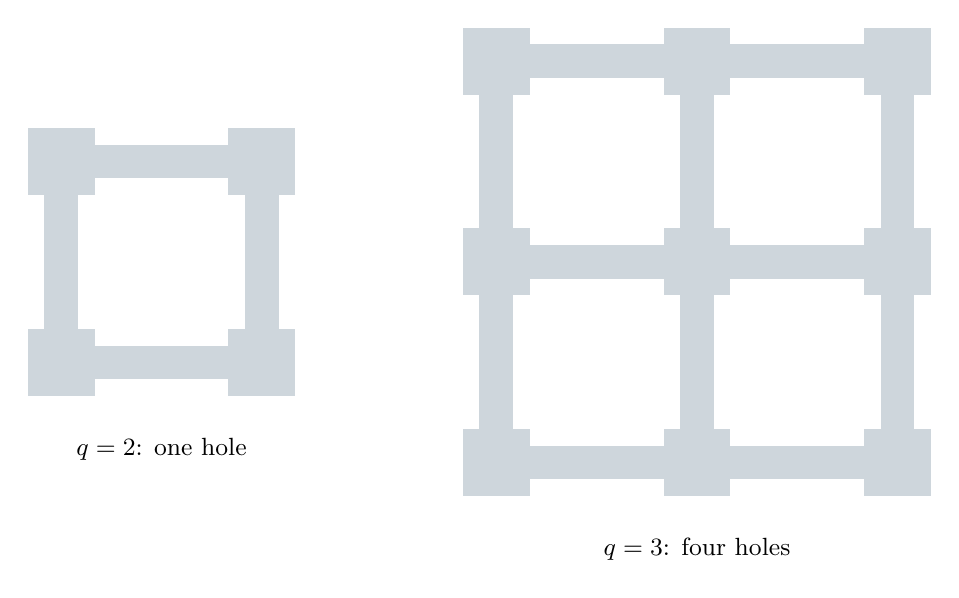
\begin{tikzpicture}[x=.85cm,y=.85cm]
 \begin{scope}[yshift=1.275cm]
  \foreach \i in {0,1}{\foreach \j in {0,1}{
    \fill[domainblue!24] ({3*\i-.5},{3*\j-.5})
      rectangle ({3*\i+.5},{3*\j+.5});}}
  \foreach \j in {0,1}{
    \fill[domainblue!24] (.5,{3*\j-.25})
      rectangle (2.5,{3*\j+.25});}
  \foreach \i in {0,1}{
    \fill[domainblue!24] ({3*\i-.25},.5)
      rectangle ({3*\i+.25},2.5);}
  \node[font=\small] at (1.5,-1.3) {$q=2$: one hole};
 \end{scope}
 \begin{scope}[xshift=5.525cm]
  \foreach \i in {0,1,2}{\foreach \j in {0,1,2}{
    \fill[domainblue!24] ({3*\i-.5},{3*\j-.5})
      rectangle ({3*\i+.5},{3*\j+.5});}}
  \foreach \i in {0,1}{\foreach \j in {0,1,2}{
    \fill[domainblue!24] ({3*\i+.5},{3*\j-.25})
      rectangle ({3*\i+2.5},{3*\j+.25});}}
  \foreach \i in {0,1,2}{\foreach \j in {0,1}{
    \fill[domainblue!24] ({3*\i-.25},{3*\j+.5})
      rectangle ({3*\i+.25},{3*\j+2.5});}}
  \node[font=\small] at (3,-1.3) {$q=3$: four holes};
 \end{scope}
\end{tikzpicture}
\caption{The actual domains $\Om_2$ and $\Om_3$, drawn at the same
physical scale. Shading is the membrane, not a center-line graph.
All white regions are outside it. Each room has side one; each
passage has length two and width $1/2$. The middle chamber in
the right-hand domain is a genuine four-port junction.}
\label{fig:grid}
\end{figure}

These domains do not tile the plane by congruent copies. Another
connected open copy with disjoint interior cannot contain a boundary
point of $\Om_q$, since its openness would force intersection with
the interior of $\Om_q$. A copy meeting a bounded hole must therefore
lie entirely inside that hole. This is impossible because $A_q\ge8>6$.
Tile boundaries cannot fill the open hole: the tiling is locally
finite by packing a fixed interior disk from each bounded copy in a
bounded enlargement, and polygon boundaries have area zero. Composing
a finite congruent partition with a plane tiling of its parent would
produce the forbidden tiling as well.

There is also a useful quantitative distinction from square-removal
criteria. Every containing rectangle $T$, in any orientation, contains
the convex hull, and therefore
\begin{equation}\label{eq:retained-fraction}
 \frac{A_q}{|T|}\le
 \frac{3q^2-2q}{(3q-2)^2}\le\frac12.
\end{equation}
The last inequality is $(q-2)(3q-2)\ge0$. A stronger comparison
allows connected nonrectangular tiling parents. Let $P$ be a bounded
connected Lipschitz plane tile containing $\Om_q$. In a tiling with
one distinguished copy $P$, every other copy is disjoint from
$\overline{\Om_q}$. A copy entering a bounded hole must stay inside
it, again contradicting $|P|\ge A_q>6$. Thus $P$ fills almost all of
every hole and
\begin{equation}\label{eq:parent-deletion}
 |P|\ge A_q+6h_q,\qquad
 \frac{|P|-A_q}{|P|}
 \ge\frac{6h_q}{A_q+6h_q}\ge\frac37.
\end{equation}
Here $8h_q-A_q=(q-2)(5q-4)\ge0$.

Suppose $P$ is a congruent $M$-subtile of a strip tile $T$,
and deleting finitely many interior-disjoint squares of side
lengths $\ell_i$ from $P$ gives $\Om_q$. Let $w$ be the strip
width and $S$ its side-face length, so $Sw=M|P|$. A square of
side $\ell_i$ has transverse width at least $\ell_i$, even
after rotation, hence $\ell_i\le w$. The planar sufficient
condition
\[
 S\ge2\sqrt2\pi M\sum_i\ell_i
\]
in \cite[Theorem~1.15 and Corollary~1.16]{JiangLin}
(numbering of arXiv version~4) would imply
\[
 |P|-A_q=\sum_i\ell_i^2
 \le w\sum_i\ell_i\le\frac{|P|}{2\sqrt2\pi},
\]
contrary to \eqref{eq:parent-deletion}.
The case $M=1$ uses the theorem directly.
This comparison concerns that stated finite-square sufficient
criterion with connected parents; it is not a classification
of all possible spectral inheritance constructions.

\subsection{Forms, cuts, and the six chamber types}

For a bounded Lipschitz cell $D$ with a relatively open
Dirichlet part $\Gamma_D$, the mixed form is
\[
 a_D(u)=\int_D\abs{\nabla u}^2\dd x,
 \qquad
 \mathcal V_D=\{u\in H^1(D):\operatorname{Tr}u=0
                  \text{ on }\Gamma_D\}.
\]
The remaining boundary has the natural Neumann condition.
Changing the status of finitely many corner points does not
change the trace condition. The form has compact resolvent,
and its eigenvalues are understood variationally. All cells
below retain Dirichlet boundary of positive length.

Dilate the network by two. Let $C=(-1,1)^2$, and let $S$
specify a subset of its four faces. For each face in $S$,
its centered segment of length one is Neumann; every other
boundary segment is Dirichlet. Denote this mixed problem by
$C_S$, and put $d=\abs S$. Let $R=(0,4)\times(0,1)$ have
Neumann conditions at its ends and Dirichlet conditions on
its long sides. The local assertion is
\begin{equation}\label{eq:local-target}
 N_{C_S}(E)+\frac d2N_R(E)
 \le\frac{(4+2d)E}{4\pi},\qquad E>0,\quad d\le4.
\end{equation}
There are six types up to the symmetries of the square,
since two adjacent and two opposite ports are different.

\begin{figure}[tb]
\centering
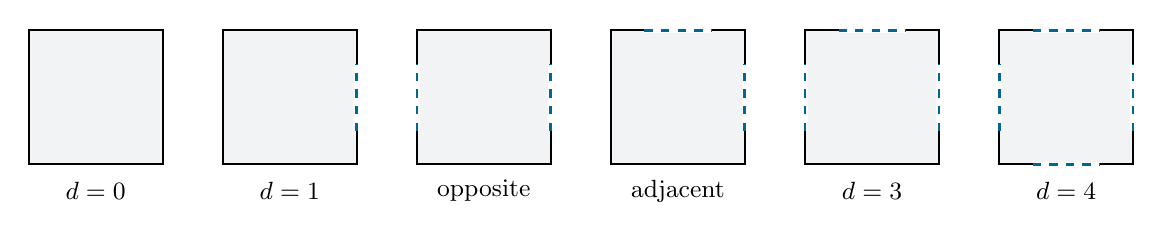
\begin{tikzpicture}[x=.85cm,y=.85cm]
 \foreach \x/\lab in {0/{$d=0$},2.9/{$d=1$},5.8/{opposite},8.7/{adjacent},11.6/{$d=3$},14.5/{$d=4$}}{
  \fill[domainblue!7] (\x,0) rectangle +(2,2);
  \draw[black,line width=.75pt] (\x,0) rectangle +(2,2);
  \node[font=\small] at (\x+1,-.4) {\lab};}
 \foreach \x in {2.9,5.8,8.7,11.6,14.5}{
  \draw[white,line width=2pt] (\x+2,.5)--(\x+2,1.5);
  \draw[portblue,dashed,line width=1pt] (\x+2,.5)--(\x+2,1.5);}
 \foreach \x in {5.8,11.6,14.5}{
  \draw[white,line width=2pt] (\x,.5)--(\x,1.5);
  \draw[portblue,dashed,line width=1pt] (\x,.5)--(\x,1.5);}
 \foreach \x in {8.7,11.6,14.5}{
  \draw[white,line width=2pt] (\x+.5,2)--(\x+1.5,2);
  \draw[portblue,dashed,line width=1pt] (\x+.5,2)--(\x+1.5,2);}
\draw[white,line width=2pt] (15,0)--(16,0);
 \draw[portblue,dashed,line width=1pt] (15,0)--(16,0);
\end{tikzpicture}
\caption{The six scaled chamber problems in \eqref{eq:local-target}.
Each square has side two. Solid black segments are Dirichlet;
dashed blue segments are Neumann windows of length one.
The three-port cell has its absent port below, as in the
cluster calculation; the final cell has four Neumann windows.}
\label{fig:cells}
\end{figure}

To see why \eqref{eq:local-target} proves the physical result,
restrict a function in $H_0^1(2\Om)$ to every chamber and
passage. Each restriction belongs to the corresponding
mixed form domain. Norms and energies add exactly, while
the direct sum allows independent traces at the cut
interfaces. The min--max principle gives
\[
 N_{2\Om}(E)
 \le\sum_{v\in V}N_{C_{S_v}}(E)+mN_R(E).
\]
Since $\sum_v d(v)=2m$, summing \eqref{eq:local-target}
bounds the right side by $(4n+4m)E/(4\pi)$. Finally,
$\lambda_k(2\Om)=\lambda_k(\Om)/4$, so this is exactly
\eqref{eq:main-result}. In particular, an absent edge has
neither a Neumann window in $C_{S_v}$ nor an assigned
passage share. The proof does not rely on boundary vertices
being negligible compared with interior vertices.

\subsection{The separable comparison}

Enlarge each Neumann window of $C_S$ to its entire face;
write $H_S$ for the resulting rectangular mixed problem.
Then $N_{C_S}(E)\le N_{H_S}(E)$. On an interval of length
two, the frequencies divided by $\pi$ are $(j+\theta)/2$,
$j\ge0$, with
\[
 \theta=0\quad(\mathrm{NN}),\qquad
 \theta=\tfrac12\quad(\mathrm{DN}),\qquad
 \theta=1\quad(\mathrm{DD}).
\]
Thus $\theta_x+\theta_y=2-d/2$. Put $E=\pi^2r^2$ and
$P=16r^2$. The chamber events are $P=a^2+b^2$, where the
allowed nonnegative numerators are
\begin{center}
\begin{tabular}{@{}llll@{}}
\toprule
Type&$a$&$b$&$d$\\\midrule
No port&$2,4,6,\ldots$&$2,4,6,\ldots$&0\\
One port&$2,4,6,\ldots$&$1,3,5,\ldots$&1\\
Opposite ports&$2,4,6,\ldots$&$0,2,4,\ldots$&2\\
Adjacent ports&$1,3,5,\ldots$&$1,3,5,\ldots$&2\\
Three ports&$1,3,5,\ldots$&$0,2,4,\ldots$&3\\
Four ports&$0,2,4,\ldots$&$0,2,4,\ldots$&4\\
\bottomrule
\end{tabular}
\end{center}
Interchanging coordinates does not affect the counts.
For $R$, the exact levels are
$\pi^2(m^2+n^2/16)$ with $m\ge1$, $n\ge0$; its events
are $P=16m^2+n^2$. The zero longitudinal mode is included.

The remainder of the proof separates two tasks. First,
actual Dirichlet segments give quantitative lower bounds
for the few levels that need improvement. Second, exact
counting and an analytic tail show that these improvements
suffice at every energy.

\section{The boundary estimates at the exceptional levels}
\label{bd:section}

We work throughout this section at the dilated scale: the chamber is
$C=(-1,1)^2$, and every present port is a centred interval of length one.
For a set $S$ of present ports, let $C_S$ denote the mixed chamber with
Neumann condition on these intervals and Dirichlet condition on the rest
of its boundary. Let $H_S$ denote the comparison chamber obtained by
extending each present Neumann interval to its entire face. The quadratic
form is the Dirichlet integral on the corresponding closed subspace of
$H^1(C)$. Consequently, increasing the Dirichlet part increases every
eigenvalue, with multiplicity. All counting functions below include
equality at the energy in question.

Only three estimates beyond this elementary comparison will be needed.
The first is a common lower bound for the ground state. The second moves
one state of the chamber with two opposite ports. The third moves both
members of a double level of the chamber with three ports. We give the
boundary calculations explicitly, including the entire spectral
complement in the last estimate.

\subsection{A common ground-state estimate}
\label{bd:ground}

Let $C_4$ be the chamber with all four Neumann windows. Every $C_S$ is a
Dirichlet strengthening of $C_4$. It therefore suffices to prove
\begin{equation}
 \lambda_1(C_4)\ge \frac{2\pi^2}{\pi^2+2}>\frac{\pi^2}{6}.
 \label{bd:ground-bound}
\end{equation}
The last strict inequality follows from $\pi^2<10$.

Consider the unit quadrant $Q=(0,1)^2$. Its prescribed Dirichlet set is
\[
 D_Q=\bigl(\{1\}\times[1/2,1]\bigr)
       \cup\bigl([1/2,1]\times\{1\}\bigr).
\]
No boundary condition on the two coordinate axes is required in the
following calculation. Define
\[
 f(t)=\mathbf 1_{(1/2,1)}(t),\qquad
 H(t)=\frac12\min(t,1-t),\qquad
 F(x,y)=\bigl(xf(y)+H(x),\;yf(x)+H(y)\bigr).
\]
Since $H'=1/2-f$ almost everywhere, $\operatorname{div}F=1$ in each
of the four half-size squares. Across each internal segment, the normal
component of $F$ is continuous: its jump is tangential. Thus the same
divergence identity holds distributionally on $Q$. The outward normal
component of $F$ is one on $D_Q$ and zero on the remaining outer boundary.

The norm of this vector field is exact. Indeed,
\[
 \int_0^1 H(t)^2\,dt=\frac1{48},\qquad
 \int_0^1 tH(t)\,dt=\frac1{16},\qquad
 \int_0^1 f(t)\,dt=\int_0^1 f(t)^2\,dt=\frac12.
\]
It follows that
\begin{equation}
 \int_Q |F|^2
 =2\left(\frac16+\frac1{16}+\frac1{48}\right)
 =\frac12.
 \label{bd:field-norm}
\end{equation}
For $u\in H^1(Q)$ whose trace vanishes on $D_Q$, integration by parts
on the four half-size squares, with cancellation of the internal normal
fluxes, gives
\[
 \int_Q u=-\int_Q F\cdot\nabla u,
 \qquad
 \left|\int_Q u\right|^2\le\frac12\int_Q|\nabla u|^2.
\]
These identities extend from smooth restrictions to $H^1(Q)$ by the
trace theorem and density. As $|Q|=1$, the mean-zero Neumann Poincar\'e
inequality on the unit square yields
\[
 \int_Q\left|u-\int_Q u\right|^2
 \le\frac1{\pi^2}\int_Q|\nabla u|^2.
\]
For completeness, its constant follows by expanding the mean-zero
function in the cosine basis: every nonconstant product mode has
eigenvalue at least $\pi^2$. The orthogonal decomposition into the mean
and the mean-zero part now gives
\[
 \int_Q|u|^2
 \le\left(\frac12+\frac1{\pi^2}\right)\int_Q|\nabla u|^2.
\]
Every admissible function on $C_4$ restricts to four functions of this
kind after reflecting their quadrants onto $Q$. Summing the four
inequalities proves \eqref{bd:ground-bound}. In particular,
\begin{equation}
 N_{C_S}^{\le}(E)=0\qquad
 \left(0<E\le\frac{\pi^2}{6}\right)
 \label{bd:no-ground}
\end{equation}
for every set of present ports.

\subsection{An anchored trace estimate and the opposite-port chamber}
\label{bd:opposite}

We first record the variational calculation used for the simple level.
Suppose a comparison problem on a rectangle has Dirichlet condition at
$x=0$. Let $\phi$ be a normalized simple eigenfunction at its $k$th
eigenvalue $\lambda_0$, and suppose the next eigenvalue is
$\lambda_0+\Delta$, where $\Delta>0$. Add a Dirichlet condition on a
measurable portion $\Gamma$ of the opposite face $x=L$, and write
\[
 g=\int_\Gamma |\phi|^2>0.
\]
Then the strengthened problem satisfies
\begin{equation}
 \lambda_k^{\mathrm{new}}
 \ge\lambda_0+\frac{\Delta g}{g+2\sqrt{\lambda_0+\Delta}}.
 \label{bd:scalar-lift}
\end{equation}

To see this, impose orthogonality to the first $k-1$ comparison
eigenfunctions on the strengthened form domain and write
\[
 u=a\phi+h,\qquad
 q(h)=\int|\nabla h|^2-\lambda_0\int|h|^2.
\]
Here $h$ is orthogonal to every comparison mode at or below
$\lambda_0$, so
\[
 q(u)=q(h),\qquad
 \|h\|_2^2\le\frac{q(h)}\Delta,\qquad
 \|\nabla h\|_2^2\le\frac{\lambda_0+\Delta}{\Delta}q(h).
\]
The identity for $q(u)$ follows from the weak eigenfunction equation for
$\phi$. Since $h$ vanishes at $x=0$, the fundamental theorem of calculus
on almost every horizontal slice gives, for every $\tau>0$,
\[
 \int_{x=L}|h|^2
 =2\operatorname{Re}\int \overline h\,\partial_xh
 \le\tau\|\partial_xh\|_2^2+\tau^{-1}\|h\|_2^2.
\]
On $\Gamma$ we have $h=-a\phi$. Consequently,
\[
 |a|^2g
 \le\frac{\tau(\lambda_0+\Delta)+\tau^{-1}}{\Delta}\,q(h),
 \qquad
 \|u\|_2^2
 \le\frac{g+\tau(\lambda_0+\Delta)+\tau^{-1}}{\Delta g}\,q(h).
\]
Taking $\tau=(\lambda_0+\Delta)^{-1/2}$ and applying the max--min
principle proves \eqref{bd:scalar-lift}. The lower comparison
eigenfunctions need not belong to the strengthened form domain. They
serve only as $L^2$ vectors defining the $k-1$ orthogonality constraints,
which is precisely what the max--min principle permits.

Now place the two opposite ports on the faces $x=\pm1$. Both the actual
chamber and its comparison problem are invariant under reflection in
each coordinate axis. Their four parity sectors are orthogonal reducing
subspaces. In the sector odd in both variables, restriction to
$Q=(0,1)^2$ gives Dirichlet conditions at $x=0$ and $y=0,1$. The
comparison condition at $x=1$ is Neumann; the actual chamber adds
Dirichlet condition on
\[
 \Gamma=\{1\}\times[1/2,1].
\]
The comparison eigenvalues in this sector are
\[
 \pi^2\bigl((m+1/2)^2+n^2\bigr),\qquad m\ge0,\quad n\ge1.
\]
Its normalized ground state, ground eigenvalue, and next gap are
\[
 \phi(x,y)=2\sin(\pi x/2)\sin(\pi y),\qquad
 \lambda_0=\frac{5\pi^2}{4},\qquad
 \Delta=2\pi^2.
\]
The normalization is on the unit quadrant, so the trace mass is
\[
 g=4\int_{1/2}^1\sin^2(\pi y)\,dy=1.
\]
Formula \eqref{bd:scalar-lift} therefore gives
\begin{equation}
 \lambda_1^{--}(C_S)
 \ge\frac{5\pi^2}{4}+\frac{2\pi^2}{1+\pi\sqrt{13}}
 >\frac{41\pi^2}{32}.
 \label{bd:opposite-lift}
\end{equation}
For the last inequality, $\pi<22/7$ and $\sqrt{13}<4$ give
$1+\pi\sqrt{13}<95/7<64$.

All other sector eigenvalues retain their comparison lower bounds.
The comparison odd--odd sector has exactly one eigenvalue between
$5\pi^2/4$ and $41\pi^2/32$, while the actual sector has none.
Accordingly,
\begin{equation}
 N_{C_S}^{\le}(E)\le N_{H_S}^{\le}(E)-1
 \qquad
 \left(\frac{5\pi^2}{4}\le E\le\frac{41\pi^2}{32}\right)
 \label{bd:opposite-count}
\end{equation}
when the two ports are opposite.

\subsection{The double level of the three-port chamber}
\label{bd:three-port}

Place the missing port on $y=-1$, so this entire face is Dirichlet.
Reflection in $x=0$ splits the actual and comparison chambers into even
and odd sectors. In the even sector, put $t=y+1$ and work on
$Q=(0,1)\times(0,2)$. The comparison problem has Neumann conditions at
$x=0,1$ and $t=2$, and Dirichlet condition at $t=0$. An orthonormal
basis is
\begin{equation}
 \psi_{mn}(x,t)=c_m\cos(m\pi x)\sin\frac{(2n+1)\pi t}{4},
 \quad
 c_0=1,\quad c_m=\sqrt2\ (m\ge1),
 \label{bd:even-basis}
\end{equation}
where $m,n\ge0$, with eigenvalues
\[
 \lambda_{mn}=\pi^2\left(m^2+\frac{(2n+1)^2}{16}\right).
\]
The three eigenvalues below $25\pi^2/16$ are
$\pi^2/16$, $9\pi^2/16$, and $17\pi^2/16$. The level
$\lambda_*=25\pi^2/16$ is double, with normalized eigenfunctions
\[
 \phi_A(x,t)=\sin(5\pi t/4),\qquad
 \phi_B(x,t)=\sqrt2\cos(\pi x)\sin(3\pi t/4).
\]
The next comparison level is $41\pi^2/16$, so the gap above the double
level is $\pi^2$.

The actual added Dirichlet boundary contains
\[
 \Gamma=\{1\}\times J,\qquad
 J=[0,1/2]\cup[3/2,2].
\]
We use only this part of the physical Dirichlet boundary; allowing
arbitrary traces on the additional Dirichlet portions gives a valid
lower comparison. Impose orthogonality to the first three comparison
even modes, and decompose any admissible function as
\begin{equation}
 \begin{aligned}
  u&=a\phi_A+b\phi_B+h,\\
  q(h)&=\int_Q|\nabla h|^2-\lambda_*\int_Q|h|^2
        \ge\pi^2\|h\|_2^2.
 \end{aligned}
 \label{bd:cluster-decomposition}
\end{equation}
Thus $h$ is orthogonal to all five comparison modes at or below
$\lambda_*$. As before, $q(u)=q(h)$.

\paragraph{The boundary moments.}
Define the two linear functionals
\[
 L_A(v)=\int_J\phi_A(1,t)v(1,t)\,dt,\qquad
 L_B(v)=\int_J\phi_B(1,t)v(1,t)\,dt.
\]
All eigenfunctions appearing here are real; these expressions are linear
also for complex $v$. For $a,n\ge0$, set
\[
 s_a(t)=\sin\frac{(2a+1)\pi t}{4},\qquad
 I_{an}=\int_J s_a(t)s_n(t)\,dt.
\]
The substitution $t\mapsto2-t$ gives
$s_a(2-t)=(-1)^a\cos((2a+1)\pi t/4)$. Therefore
\begin{equation}
 I_{an}=
 \begin{cases}
 \displaystyle\int_0^{1/2}\cos\frac{(a-n)\pi t}{2}\,dt,
       &a+n\ \text{even},\\[6pt]
 \displaystyle-\int_0^{1/2}\cos\frac{(a+n+1)\pi t}{2}\,dt,
       &a+n\ \text{odd}.
 \end{cases}
 \label{bd:moment-integrals}
\end{equation}
In particular,
\[
 I_{11}=I_{22}=\frac12,\qquad
 I_{20}=\frac1\pi,\qquad I_{10}=-\frac1\pi,\qquad
 I_{12}=I_{21}=0.
\]
Since $\phi_B(1,t)=-\sqrt2\,s_1(t)$, the matrix of these functionals
on the double eigenspace is exactly
\begin{equation}
 \begin{pmatrix}
  L_A(\phi_A)&L_A(\phi_B)\\
  L_B(\phi_A)&L_B(\phi_B)
 \end{pmatrix}
 =D:=\begin{pmatrix}1/2&0\\0&1\end{pmatrix}.
 \label{bd:trace-matrix}
\end{equation}
The trace condition on $u$ consequently implies
\begin{equation}
 L(h):=\begin{pmatrix}L_A(h)\\L_B(h)\end{pmatrix}
 =-D\begin{pmatrix}a\\b\end{pmatrix}.
 \label{bd:moment-constraint}
\end{equation}

The functions $s_n$, $n\ge0$, form an orthonormal basis of $L^2(0,2)$.
Applying Parseval to $\mathbf1_Js_a$ gives
\[
 \sum_{n\ge0}I_{an}^2=\int_J s_a^2=\frac12.
\]
Subtracting the three explicitly computed terms yields the exact
complement identity
\begin{equation}
 \sum_{n\ge3}I_{an}^2=\frac14-\frac1{\pi^2},
 \qquad a=1,2.
 \label{bd:parseval}
\end{equation}

\paragraph{The complete high-mode bound.}
Let $\mathcal I$ consist of the pairs $(m,n)$ with
$\lambda_{mn}>\lambda_*$. The positive boundary Gram matrix is
\begin{equation}
 G=\sum_{(m,n)\in\mathcal I}
 \frac{L(\psi_{mn})L(\psi_{mn})^*}{\lambda_{mn}-\lambda_*}.
 \label{bd:gram-definition}
\end{equation}
Here the star denotes conjugate transpose. The diagonal estimates below
prove convergence of this full series. Weighted Cauchy--Schwarz in the
expansion of $h$ then gives
\begin{equation}
 |z^*L(h)|^2\le (z^*Gz)\,q(h)
 \qquad(z\in\mathbb C^2).
 \label{bd:gram-cauchy}
\end{equation}
One may first apply this inequality to finite expansions. Their spectral
partial sums converge in the form norm, and the trace functionals are
continuous in that norm, so the displayed inequality follows for every
$h$ in \eqref{bd:cluster-decomposition}.

At $x=1$ the boundary values of $\psi_{mn}$ are
$c_m(-1)^m s_n$. Hence
\begin{equation}
 G_{AA}=\frac1{\pi^2}\sum_{n\ge0}I_{2n}^2H_n,
 \qquad
 G_{BB}=\frac2{\pi^2}\sum_{n\ge0}I_{1n}^2H_n,
 \label{bd:gram-diagonals}
\end{equation}
where the following expressions remove precisely the five low modes:
\begin{equation}
 \begin{aligned}
  H_0&=\sum_{m\ge2}\frac2{m^2-3/2},\qquad
  H_1=\sum_{m\ge2}\frac2{m^2-1},\qquad
  H_2=\sum_{m\ge1}\frac2{m^2},\\
  H_n&=\frac1{\beta_n}+\sum_{m\ge1}\frac2{m^2+\beta_n}
        \quad(n\ge3),\qquad
  \beta_n=\frac{(2n+1)^2-25}{16}\ge\frac32.
 \end{aligned}
 \label{bd:high-sums}
\end{equation}
The first three are bounded or evaluated by
\begin{equation}
 H_0\le\frac{16}{5}\left(\frac{\pi^2}{6}-1\right)
       <\frac{32}{15},\qquad
 H_1=\frac32,\qquad H_2=\frac{\pi^2}{3}.
 \label{bd:first-high-sums}
\end{equation}
For $H_0$ we used $m^2-3/2\ge(5/8)m^2$ for $m\ge2$.
For $H_1$ the identity
$2/(m^2-1)=1/(m-1)-1/(m+1)$ telescopes. For $n\ge3$, comparison of a
decreasing positive summand with its integral gives
\begin{equation}
 H_n\le\frac1{\beta_n}
       +2\int_0^\infty\frac{dx}{x^2+\beta_n}
 =\frac1{\beta_n}+\frac\pi{\sqrt{\beta_n}}
 \le\frac23+\pi\sqrt{\frac23}<\frac{23}{7}.
 \label{bd:infinite-high-sums}
\end{equation}
The last comparison uses $\sqrt{2/3}<5/6$ and $\pi<22/7$.

Put
\[
 A=\frac{H_0}{\pi^4}
     +\frac{23}{7\pi^2}\left(\frac14-\frac1{\pi^2}\right).
\]
The bounds $\pi>25/8$ and $\pi^2<10$ give
\begin{equation}
 A<\left(\frac{64}{625}\right)^2\frac{32}{15}
       +\frac{64}{625}\frac{23}{7}\frac3{20}
   =\frac{2987504}{41015625}<\frac{73}{1000}.
 \label{bd:rational-A}
\end{equation}
Using \eqref{bd:parseval} in \eqref{bd:gram-diagonals}, we obtain
\begin{equation}
 G_{AA}<\frac1{12}+\frac{73}{1000}=\frac{469}{3000},\qquad
 G_{BB}<2\left(\frac{73}{1000}+\frac3{8\pi^2}\right)
       <\frac{557}{2500}.
 \label{bd:gram-rational}
\end{equation}
No off-diagonal estimate is needed. The largest eigenvalue of the
positive matrix $D^{-1}GD^{-1}$ is at most its trace, and
\[
 \operatorname{Tr}(D^{-1}GD^{-1})
 =4G_{AA}+G_{BB}<\frac{6361}{7500}<\frac{17}{20}.
\]
Congruence by $D$ gives the uniform matrix bound
\begin{equation}
 G\le\frac{17}{20}D^2.
 \label{bd:gram-majorant}
\end{equation}
Every term of the infinite spectral complement has entered these
estimates. In particular, no truncation of a positive tail is being used
as an upper bound.

\paragraph{The spectral conclusion, including multiplicity.}
Let $v=(a,b)^{\mathsf T}$. If $v\ne0$, use $z=D^{-1}v$ in
\eqref{bd:gram-cauchy}, together with
\eqref{bd:moment-constraint} and \eqref{bd:gram-majorant}. This gives
\[
 |v|^4\le\frac{17}{20}|v|^2q(h),\qquad
 |a|^2+|b|^2\le\frac{17}{20}q(h).
\]
The second inequality is also valid when $v=0$. Combining it with the
gap in \eqref{bd:cluster-decomposition}, we find
\[
 \|u\|_2^2=|a|^2+|b|^2+\|h\|_2^2
 \le\left(\frac{17}{20}+\frac1{\pi^2}\right)q(h).
\]
The three orthogonality conditions imposed above are legitimate in the
max--min formula for the fourth actual even eigenvalue. We conclude that
\begin{equation}
 \begin{aligned}
  \lambda_4^{+}(C_S)
  &\ge\frac{25\pi^2}{16}+\frac{20\pi^2}{17\pi^2+20}\\
  &>\frac{25\pi^2}{16}+\frac{2\pi^2}{19}
   =\frac{507\pi^2}{304}>\frac{5\pi^2}{3}>\frac{53\pi^2}{32}.
 \end{aligned}
 \label{bd:double-lift}
\end{equation}
Here $\pi^2<10$, $507/304-5/3=1/912$, and
$5/3-53/32=1/96$ prove the strict comparisons. This is a uniform estimate for
the Rayleigh quotient on the constrained space. Both members of the
double level, and every later even eigenvalue, therefore lie strictly
above $53\pi^2/32$.

For the odd sector, the comparison eigenvalues are
\[
 \pi^2\left((m+1/2)^2+\frac{(2n+1)^2}{16}\right),
 \qquad m,n\ge0.
\]
Exactly two lie at or below $53\pi^2/32$, namely $5\pi^2/16$ and
$13\pi^2/16$; the next is $29\pi^2/16$. Thus the actual even sector
contributes at most three states and the odd sector at most two through
$53\pi^2/32$. On the interval starting at $25\pi^2/16$, the full
comparison chamber has exactly seven states. Consequently,
\begin{equation}
 N_{C_S}^{\le}(E)\le5=N_{H_S}^{\le}(E)-2
 \qquad
 \left(\frac{25\pi^2}{16}\le E\le\frac{53\pi^2}{32}\right)
 \label{bd:three-port-count}
\end{equation}
for the three-port chamber.

In the event coordinate $P=16E/\pi^2$, the preceding estimates allow
one to remove any comparison ground state below $P=8/3$, one state of
the opposite-port chamber for $20\le P<41/2$, and two states of the
three-port chamber for $25\le P<53/2$. The estimates remain valid at
the upper endpoints. The finite count may nevertheless cease using a
correction there, provided the resulting jump of the chosen upper bound
is checked at that endpoint.

\section{An elementary estimate for the counting-function tail}
\label{sec:counting-tail}

The boundary estimates handle only a few low levels. To control every
remaining energy, we first obtain a uniform lower bound on the fractional
parts lost when a quarter-circle sum is replaced by its integral. The
uniformity in both sampling phases is useful here: the chamber types
have different Dirichlet and Neumann conditions, but they can all be treated
by the same estimate.

\subsection{Fractional parts in consecutive blocks}

Write $\{z\}=z-\lfloor z\rfloor$. For an integer $K\ge2$, set
\[
 M_K(\alpha)=\min_{t\in\mathbb R}
       \sum_{k=0}^{K-1}\{t-k\alpha\},
 \qquad C_K=\frac{K(K-1)}2.
\]
As $t$ runs through a period, the sum increases linearly between its
downward jumps. Its minimum therefore occurs when at least one fractional
part is zero, including when several jumps coincide. Consequently
\begin{equation}
 M_K(\alpha)=\min_{0\le j<K}
       \sum_{k=0}^{K-1}\{(j-k)\alpha\},
 \qquad 0\le M_K(\alpha)\le\frac{K-1}{2}.
 \label{eq:block-minimum}
\end{equation}
For the upper bound, average the $K$ candidate sums. Each unordered pair
of distinct indices contributes $\{z\}+\{-z\}$, which is either zero or
one; their total is at most $C_K$.

Although a fractional part is discontinuous, this minimized sum is
$C_K$-Lipschitz. Indeed, if $\beta\ge\alpha$, choose a minimizing phase
for $\beta$ and use
\[
 \{z+h\}\le\{z\}+h\qquad(h\ge0)
\]
with $h=k(\beta-\alpha)$. This gives
$M_K(\alpha)\le M_K(\beta)+C_K(\beta-\alpha)$.
Reversing the order of the $K$ terms and translating the phase shows
$M_K(-\alpha)=M_K(\alpha)$; applying the same inequality to
$-\beta\le-\alpha$ gives the reverse bound. Thus
\begin{equation}
 |M_K(\beta)-M_K(\alpha)|\le C_K|\beta-\alpha|.
 \label{eq:block-lipschitz}
\end{equation}
This argument includes rational slopes and repeated phases.

For $T>0$ and $a>0$, define
\[
 f_T(t)=\sqrt{T^2-t^2},\qquad
 g_a(x)=\frac{ax}{\sqrt{1-x^2}},\qquad
 x_G=\frac{G}{\sqrt{a^2+G^2}},
\]
where $G>0$, and put
\[
 A(a,K,G)=\frac1K\int_0^{x_G}M_K(g_a(x))\,dx.
\]
For every $\theta\in[0,1]$ and every $\eta\in\mathbb R$, the complete
sampled fractional-part sum satisfies
\begin{equation}
 \sum_{\substack{j\ge0\\j+\theta\le T}}
       \{a f_T(j+\theta)-\eta\}
 \ge T A(a,K,G)-\frac{K^2G}{8}-\frac K2.
 \label{eq:fractional-block}
\end{equation}

Write $h(t)=a f_T(t)$ and first consider a block $I=[b,b+K]$ contained
in $[0,Tx_G]$, with samples $s_k=b+k+\tfrac12$, $0\le k<K$.
For any $t\in I$, the tangent line to the concave function $h$ gives
\[
 h(s_k)=h(t)+h'(t)(s_k-t)-e_k(t),\qquad e_k(t)\ge0.
\]
Its values at successive samples form an arithmetic progression with
drop $g_a(t/T)$. Since $\{z-e\}\ge\{z\}-e$ for $e\ge0$,
\[
 \sum_{k=0}^{K-1}\{h(s_k)-\eta\}
 \ge M_K(g_a(t/T))-\sum_{k=0}^{K-1}e_k(t).
\]
Average over $t\in I$. Put $q(s)=-h''(s)\ge0$, write $x=s-b$, and
let $n$ be the number of sample points at or to the left of $s$.
Changing the order of integration in the nonnegative tangent remainders
gives
\[
 \frac1K\int_I\sum_ke_k(t)\,dt
 =\int_I w_K(s-b)q(s)\,ds,
\]
where
\begin{equation}
 \begin{aligned}
 w_K(x)
 &=\frac{x}{K}\sum_{s_k\ge s}(s_k-s)
       +\frac{K-x}{K}\sum_{s_k\le s}(s-s_k)\\
 &=\frac{x(K-x)}2-\frac{(n-x)^2}{2}
 \le\frac{K^2}{8}.
 \end{aligned}
 \label{eq:tangent-block-kernel}
\end{equation}
Indeed, the left and right distance sums are $nx-n^2/2$ and
$K^2/2-Kx+nx-n^2/2$. The formula also holds at a sampled point, where
the corresponding summand is zero. Therefore the complete block obeys
\[
 \begin{split}
 \sum_k\{h(s_k)-\eta\}
 &\ge\frac1K\int_I M_K(g_a(t/T))\,dt\\
 &\quad-\frac{K^2}{8}
       \bigl[g_a((b+K)/T)-g_a(b/T)\bigr].
 \end{split}
\]
For the prescribed sample phase, take $j_0=0$ when $\theta\ge1/2$ and
$j_0=1$ otherwise. Then $b=j_0+\theta-1/2\in[0,1)$, so consecutive
blocks starting at $b$ are centered on original samples. Retain all
complete blocks ending at or before $Tx_G$. Their derivative increments
telescope to at most $G$. The omitted initial and final lengths total
less than $K+1$. By \eqref{eq:block-minimum}, the corresponding loss
from the integral divided by $K$ is less than
$(K+1)(K-1)/(2K)<K/2$. All discarded fractional parts are nonnegative.
If there is no complete block, $Tx_G<K+1$ and the same bound gives
$TA<K/2$ directly. This proves \eqref{eq:fractional-block} for all
phases, small $T$, and empty sample sets. All differentiations occur
below $Tx_G<T$, where the circle is smooth.

For degrees at most three, use
\begin{align}
 A(1,6,2)&\ge\frac{860001557153}{3276800000000}>
                 \frac{13}{50},\\
 A(4,4,4)&\ge\frac{138748241337}{819200000000}>
                 \frac{169}{1000}.
 \label{eq:block-integrals}
\end{align}
These are exact lower sums certified by the Lipschitz bound. The integer
construction and its complete parameters are given in
Appendix~\ref{app:certificates}. Inserting them into
\eqref{eq:fractional-block} gives, respectively,
\begin{equation}
 F_H\ge\frac{13}{25}r-12,
 \qquad F_R\ge\frac{169}{1000}r-10,
 \label{eq:fractional-losses}
\end{equation}
for chamber rows with $T=2r$, $a=1$, and corridor rows with $T=r$, $a=4$.

\subsection{Shifted quarter-circle sums and the common tail}

Let $c=\sqrt{2/27}$. The following elementary estimate applies to
$\theta=0,\tfrac12,1$:
\begin{equation}
 \sum_{\substack{j\ge0\\j+\theta\le T}} f_T(j+\theta)
 \le\frac{\pi T^2}{4}+\left(\frac12-\theta\right)T
          +c\sqrt T.
 \label{eq:shifted-circle}
\end{equation}
For $\theta=1$, write $M=\lfloor T\rfloor$ and $s=T-M$. The
trapezoidal inequality for the concave function $f_T$, followed by the
chord bound on $[M,T]$, gives
\[
 \begin{split}
 \sum_{m=1}^{M}f_T(m)
 &\le\frac{\pi T^2}{4}-\frac T2+
            \frac{f_T(M)}2-\int_M^T f_T(t)\,dt\\
 &\le\frac{\pi T^2}{4}-\frac T2+
            \frac{1-s}{2}\sqrt{2Ts}.
 \end{split}
\]
The last factor is at most $c\sqrt T$, since
$\max_{0\le s\le1}(1-s)\sqrt{s}=2/(3\sqrt3)$.
When $M=0$, the initial trapezoidal identity has both sides zero before
the tail is inserted, so the argument still applies. The case $\theta=0$
adds $f_T(0)=T$. For $\theta=\tfrac12$, start the trapezoids at
$1/2$. The initial correction is nonpositive because
$\int_0^{1/2}f_T(t)\,dt\ge f_T(1/2)/2$; the last correction is the
same expression with $s$ the distance from the final sampled point to
$T$. If there is no half-integer sample, the right-hand side is positive
and the assertion is immediate.

Recall the dilated chamber $C_S$, with $d=|S|$ present ports, and the
$4$-by-$1$ corridor $R$. Relax each present-port face of $C_S$ entirely
to Neumann, keeping every missing-port face entirely Dirichlet, and call
the resulting rectangle $H_S$. In one coordinate its frequencies, in
units of $\pi$, are $(j+\theta)/2$, $j\ge0$, where
\[
 \theta=0,\ \tfrac12,\ 1
 \quad\hbox{for NN, DN, DD, respectively}.
\]
The two coordinate phases satisfy
$\theta_x+\theta_y=2-d/2$. Throughout this calculation
\begin{equation}
 E=\pi^2r^2,
 \qquad P=16r^2,
 \label{eq:compact-energy-coordinate}
\end{equation}
and all counts include equality at the threshold.

With $T=2r$, exact counting in each horizontal row yields
\[
 N_{H_S}^{\le}(E)=\sum_{\substack{j\ge0\\j+\theta_y\le T}}
 \left[f_T(j+\theta_y)+1-\theta_x
       -\{f_T(j+\theta_y)-\theta_x\}\right].
\]
The summand is $\lfloor f_T(j+\theta_y)-\theta_x\rfloor+1$.
Since $0\le\theta_x\le1$ and $f_T\ge0$, it is never negative and
equals the exact number of allowed nonnegative indices. In particular,
a row below the first DN frequency contributes zero; a zero-radius NN
row contributes one; a zero-radius DD row contributes zero. There is no
endpoint convention to repair afterward.

The number of rows is at most $T+1-\theta_y$. Multiplying this bound by
$1-\theta_x\ge0$ and using \eqref{eq:shifted-circle}, with $F_H$ the
fractional-part sum just displayed, gives
\begin{equation}
 N_{H_S}^{\le}(E)\le\pi r^2+(d-1)r+c\sqrt{2r}+1-F_H.
 \label{eq:chamber-tail-bookkeeping}
\end{equation}
Here the constant $(1-\theta_x)(1-\theta_y)$ has only been enlarged to
one. Likewise the corridor spectrum gives the exact row formula
\[
 N_R^{\le}(E)=\sum_{m=1}^{\lfloor r\rfloor}
       \left[4f_r(m)+1-\{4f_r(m)\}\right],
\]
and hence
\begin{equation}
 N_R^{\le}(E)\le\pi r^2-r+4c\sqrt r-F_R.
 \label{eq:corridor-tail-bookkeeping}
\end{equation}
The two sums $F_H,F_R$ have exactly the phases covered by
\eqref{eq:fractional-losses}.

Subtracting the local area budget from the sum of
\eqref{eq:chamber-tail-bookkeeping} and $d/2$ times
\eqref{eq:corridor-tail-bookkeeping} bounds the excess by
\[
 \left(\frac d2-1\right)r+
 c(\sqrt2+2d)\sqrt r+1-F_H-\frac d2F_R.
\]
After \eqref{eq:fractional-losses}, this is at most
\[
 \left(\frac{831d}{2000}-\frac{38}{25}\right)r+
 c(\sqrt2+2d)\sqrt r+13+5d.
\]
Every coefficient increases with $d$. Thus for $0\le d\le3$, using
$c<3/11$ and $\sqrt2<10/7$, the excess is bounded above by
\[
 -\frac{547}{2000}r+\frac{156}{77}\sqrt r+28.
\]
At $r=800$, the bound $\sqrt{800}<29$ makes this at most
$-50838/385<0$. After division by $r$, both positive terms decrease.
We have therefore proved the common tail
\begin{equation}
 \begin{aligned}
  N_{C_S}^{\le}(\pi^2r^2)+\frac d2N_R^{\le}(\pi^2r^2)
  &\le N_{H_S}^{\le}(\pi^2r^2)+\frac d2N_R^{\le}(\pi^2r^2)\\
  &\le\left(1+\frac d2\right)\pi r^2
       \qquad(r\ge800,\ d\le3).
 \end{aligned}
 \label{eq:compact-tail}
\end{equation}
Only form-domain inclusion was used in replacing $C_S$ by $H_S$.

The four-port chamber requires larger blocks. The same exact lower-sum
construction, with the parameters specified in
Appendix~\ref{app:certificates}, gives
\begin{align}
 A(1,13,3)&\ge\frac{37632015538794073}{106496000000000000}
                >\frac{353}{1000},\nonumber\\
 A(4,7,8)&\ge\frac{32022499598134509}{114688000000000000}
                >\frac{279}{1000}.
 \label{eq:degree-four-integrals}
\end{align}
Thus \eqref{eq:fractional-block} gives, for the same chamber and
corridor fractional sums,
\[
 F_H\ge\frac{353}{500}r-\frac{559}{8},\qquad
 F_R\ge\frac{279}{1000}r-\frac{105}{2}.
\]
The degree-four specialization of the preceding row bookkeeping bounds
the excess $N_H^{\le}(\pi^2r^2)+2N_R^{\le}(\pi^2r^2)-3\pi r^2$
by
\[
 r+c(\sqrt2+8)\sqrt r+1-F_H-2F_R
 \le-\frac{33}{125}r+\frac{18}{7}\sqrt r+\frac{1407}{8},
\]
where $c(\sqrt2+8)<18/7$. At $r=1024$ this last expression equals
$-85227/7000<0$. Again, after division by $r$, the positive terms
decrease. If $C_4$ denotes the actual four-port chamber and $H$ its fully
Neumann relaxation, we obtain
\begin{equation}
 \begin{aligned}
 N_{C_4}^{\le}(\pi^2r^2)+2N_R^{\le}(\pi^2r^2)
 &\le N_H^{\le}(\pi^2r^2)+2N_R^{\le}(\pi^2r^2)\\
 &\le3\pi r^2\qquad(r\ge1024).
 \end{aligned}
 \label{eq:degree-four-tail}
\end{equation}
The finite interval for this last chamber will be completed after the
five degree-at-most-three types.

\section{The finite certificate for degrees at most three}
\label{sec:finite-closure}

The remaining interval is finite, but its verification must still retain
all multiplicities and all real energy thresholds. In the coordinate
$P=16r^2$, every separated chamber event is $P=a^2+b^2$, with the five
numerator pairs listed in Section~\ref{sec:geometry}. Corridor events
are $P=a^2+16b^2$, with $a\ge0$ and $b\ge1$ integers. Repeated
representations are distinct eigenfunctions and are counted separately.

Write $N_H=N_{H_S}^{\le}(\pi^2P/16)$ and
$N_R=N_R^{\le}(\pi^2P/16)$ when the energy argument is suppressed.
The exact rational comparison
\begin{equation}
 16\cdot33102\,(2N_H+dN_R)
 \le103993(2+d)P
 \label{eq:compact-rational-test}
\end{equation}
implies the desired local estimate because $\pi>103993/33102$.
Scanning every union event through
$P_*=16\cdot800^2=10240000$, its complete list of failures before any
boundary correction is
\begin{center}
\begin{tabular}{c|r|r|r}
type & $P$ & $N_H$ & $N_R$\\ \hline
$d=2$, adjacent & $2$ & $1$ & $0$\\
$d=2$, opposite & $20$ & $5$ & $3$\\
$d=3$ & $1$ & $1$ & $0$\\
$d=3$ & $25$ & $7$ & $4$
\end{tabular}
\end{center}
The scan is specified completely in Appendix~\ref{app:certificates}.
This table locates the needed boundary information; the corrected
verification below, including the correction endpoints, is what proves
the finite interval.

Use the actual-cell boundary estimates
\eqref{bd:ground-bound}, \eqref{bd:opposite-count}, and
\eqref{bd:three-port-count}: the ground level is greater than $\pi^2/6$;
the indicated opposite-port sector level is greater than $41\pi^2/32$;
and the two degree-three cluster levels are greater than $53\pi^2/32$.
Define the number of removed chamber states by
\begin{equation}
 \begin{array}{ll}
 c_S(P)=0, & d=0,1,\\[2pt]
 c_S(P)=\mathbf1_{[20,41/2)}(P), & d=2\text{, opposite},\\[2pt]
 c_S(P)=\mathbf1_{\{P<8/3\}}\min\{1,N_H\},
       &d=2\text{, adjacent},\\[2pt]
 c_S(P)=\mathbf1_{\{P<8/3\}}\min\{1,N_H\}
          +2\mathbf1_{[25,53/2)}(P), &d=3.
 \end{array}
 \label{eq:compact-corrections}
\end{equation}
The ground correction is used only
after its relaxed state has appeared; there is exactly one such state
in the stated interval. The sector comparisons, with the other sectors
left at their relaxed bounds, give
\[
 N_{C_S}^{\le}(\pi^2P/16)\le N_H-c_S(P).
\]
All left endpoints in \eqref{eq:compact-corrections} are included.
At the three right endpoints the corrections are conservatively set to
zero, even though the spectral lifts are strict there as well.

For the corrected scan, replace $2N_H+dN_R$ in
\eqref{eq:compact-rational-test} by
\[
 U_S(P)=2\bigl(N_H-c_S(P)\bigr)+dN_R,
\]
and record the integer or rational margin
\begin{equation}
 \mathcal M_S(P)=103993(2+d)P-16\cdot33102\,U_S(P).
 \label{eq:compact-margin}
\end{equation}
Every actual union event through $P_*$ has positive margin. The complete
event totals and minimum margins are
\begin{center}
\begin{tabular}{c|r|r|r}
type & actual union events & minimum margin & at $P$\\ \hline
$d=0$ & $1028343$ & $604624$ & $8$\\
$d=1$ & $1390540$ & $500631$ & $5$\\
$d=2$, opposite & $1028657$ & $440576$ & $80$\\
$d=2$, adjacent & $1402109$ & $222632$ & $26$\\
$d=3$ & $1391119$ & $198901$ & $89$
\end{tabular}
\end{center}
These totals include corridor events when $d=0$; including them is
harmless and makes the enumeration rule uniform. The additional
correction-reset events give
\begin{center}
\begin{tabular}{c|c|r|c}
type & $P$ & $U_S(P)$ & $\mathcal M_S(P)$\\ \hline
$d=2$, opposite & $41/2$ & $16$ & $53314$\\
$d=2$, adjacent & $8/3$ & $2$ & $149984/3$\\
$d=3$ & $8/3$ & $2$ & $981928/3$\\
$d=3$ & $53/2$ & $26$ & $17281/2$
\end{tabular}
\end{center}
Since all actual events have integer $P$, the counts at these
noninteger thresholds equal the cumulative counts at $\lfloor P\rfloor$.
The corrections are evaluated at the threshold itself, so they have
already switched off.

Between two consecutive actual or reset events the corrected upper
count is constant, while the area budget increases with $P$. Before
the first event it is zero. This proves the local comparison for every
real $0<P\le P_*$, not just at separated eigenvalues. The endpoint
$P_*$ itself is a corridor event and is included in the scan; it also
belongs to \eqref{eq:compact-tail}. Thus the finite and infinite ranges
join without a missing energy, and together yield
\begin{equation}
 N_{C_S}^{\le}(E)+\frac d2N_R^{\le}(E)
 \le\frac{(4+2d)E}{4\pi}
 \qquad(E>0,\ d\le3).
 \label{eq:compact-final-module}
\end{equation}

This completes five of the six local comparisons. The next section
supplies the four-port estimate and then sums the local bounds over
the physical network, including all interface shares and multiplicities.

\section{The four-port chamber}
\label{sec:degree-four}

The remaining chamber has four centered Neumann windows and retains
Dirichlet boundary at all four corners. Denote it by $C_4$, and denote
the fully Neumann square by $H$. The estimate to be proved is
\begin{equation}
 N_{C_4}^{\le}(E)+2N_R^{\le}(E)\le\frac{3E}{\pi}
 \qquad(E>0).
 \label{df:local-result}
\end{equation}
The fully Neumann comparison alone has several low-energy deficits.
We repair these by retaining moments of the actual Dirichlet trace.
The resulting matrices have order at most six; their complements are
bounded analytically, rather than omitted.

\subsection{A finite block with a complete spectral complement}

Put
\[
 X_m(x)=\cos\frac{m\pi(x+1)}2,\qquad
 \Psi_{mn}(x,y)=X_m(x)X_n(y),\qquad
 q_{mn}=\frac{m^2+n^2}{4},
\]
for $m,n\ge0$, and let $d_0=2$, $d_m=1$ for $m\ge1$.
Thus the unnormalized Neumann basis has squared norms
$\nu_{mn}=d_md_n$ and energies $\pi^2q_{mn}$.
Let $\Gamma$ be the union of the Dirichlet portions of the four faces.
On each face its tangential coordinate belongs to
$[-1,-1/2]\cup[1/2,1]$.

Fix $e>0$ outside the Neumann spectrum. From the modes with $q_{mn}<e$
select $k$ mutually orthogonal vectors $g_1,\ldots,g_k$, each contained
in a single Neumann eigenspace, of respective dimensionless energies
$q_1,\ldots,q_k$. Write $M$ for the number of all Neumann modes below
$e$, including multiplicity. Impose orthogonality to the remaining
$M-k$ low directions. Every function in this constrained actual form
domain then has the expansion
\[
 u=\sum_{j=1}^k a_jg_j+h,
 \qquad
 h\in\overline{\operatorname{span}}\{\Psi_{mn}:q_{mn}>e\}.
\]
Define the boundary moments and matrices by
\begin{align*}
 L_i(v)&=\int_\Gamma \overline{g_i}\,\operatorname{Tr}v\,\dd s,
 &D_{ij}&=L_i(g_j),\\
 W_{ij}&=\delta_{ij}(e-q_j)\norm{g_j}_{L^2(C)}^2,
 &B_{mn,i}&=L_i(\Psi_{mn}),\\
 S_e&=\sum_{q_{mn}>e}
       \frac{B_{mn}B_{mn}^*}{\nu_{mn}(q_{mn}-e)}.
\end{align*}
Here $D$ is a boundary Gram matrix and $W$ is positive diagonal.
All vectors used below are real; the adjoints permit the same argument
for complex form functions. Set
\[
 Q_e(v)=\pi^{-2}\int_C\abs{\nabla v}^2\,\dd x-e\norm v_{L^2(C)}^2.
\]
The trace condition and orthogonality give
\[
 L(h)=-Da,\qquad Q_e(u)=Q_e(h)-a^*Wa.
\]
Weighted Cauchy--Schwarz in the complete high-mode expansion yields
\begin{equation}
 \abs{z^*Da}^2\le (z^*S_ez)Q_e(h)
 \qquad(z\in\mathbb C^k).
 \label{df:moment-cauchy}
\end{equation}
The tail bound below proves convergence of $S_e$. The expansion also
converges in $H^1$, so continuity of the trace justifies this calculation
first for partial sums and then for every form function.

Suppose an explicit positive matrix $\overline S$ satisfies
$S_e\le\overline S$ and
\begin{equation}
 T=DW^{-1}D-\overline S>0.
 \label{df:matrix-test}
\end{equation}
This forces $D$ to be nonsingular: a vector in its kernel would give
$z^*Tz=-z^*\overline Sz\le0$. Hence $D>0$ and, by congruence and
inversion,
\[
 D^{-1}\overline S D^{-1}<W^{-1},\qquad
 K:=D\overline S^{-1}D>W.
\]
Maximizing \eqref{df:moment-cauchy} over $z$ gives
$Q_e(h)\ge a^*Ka$. There is also a positive Neumann spectral gap
$\delta_e=\min_{q_{mn}>e}(q_{mn}-e)$, giving
$Q_e(h)\ge\delta_e\norm h^2$. Choose $\theta>0$ small enough that
$(1-\theta)K-W>0$. Then
\[
 Q_e(u)\ge
 a^*\bigl((1-\theta)K-W\bigr)a
 +\theta\delta_e\norm h^2.
\]
This is uniformly positive relative to $\norm u^2$ on the constrained
subspace. The max--min principle, with precisely $M-k$ orthogonality
conditions, therefore proves
\begin{equation}
 \lambda_{M-k+1}(C_4)>\pi^2e,
 \qquad N_{C_4}^{\le}(\pi^2e)\le M-k.
 \label{df:block-cap}
\end{equation}
In particular, equality at the target energy is excluded. This is a
lower-bound argument on the actual form domain, not an upper-bound
Ritz approximation.

\subsection{Explicit entries and the infinite high-mode tail}

The tangential integrals needed for every entry are
\[
 J_{ab}=\int_{[-1,-1/2]\cup[1/2,1]}X_a(s)X_b(s)\,\dd s.
\]
Direct integration gives
\begin{equation}
 J_{ab}=\begin{cases}
 0,&a+b\text{ odd},\\[2pt]
 \displaystyle 2\left[
 \frac{\sin((a-b)\pi/4)}{(a-b)\pi}
 +\frac{\sin((a+b)\pi/4)}{(a+b)\pi}\right],
 &a+b\text{ even}.
 \end{cases}
 \label{df:J}
\end{equation}
The quotient with zero denominator is assigned its limit $1/4$.
For equal parity the sine values are $0,1,-1$, so $J_{ab}$ is a
rational number plus a rational multiple of $1/\pi$.
For a single selected mode $g_i=\Psi_{ab}$ the four faces give
\begin{equation}
 B_{mn,i}=
 \bigl(1+(-1)^{a+m}\bigr)J_{bn}
 +\bigl(1+(-1)^{b+n}\bigr)J_{am}.
 \label{df:coupling}
\end{equation}
Linearity gives the entries for combinations of modes, and
$D_{ij}=L_i(g_j)$ uses the same formula.

For completeness, let $f$ be any linear combination of the boundary
densities $g_i|_\Gamma$, and extend its restriction to each face by zero
on the Neumann window. Write $A_n$ for its tangential cosine moment on
one face. One-dimensional Parseval gives
\[
 \sum_{n\ge0}\frac{\abs{A_n}^2}{d_n}
 =\int_{-1}^1\abs f^2\,\dd s.
\]
In the normalized two-dimensional basis, a single face contributes
$A_n/\sqrt{d_md_n}$ up to a sign. For a cutoff $B$ with
$\beta=(B+1)^2-4e>0$, split the omitted pairs into the normal-index
tail $m>B$ and the tangential-index tail $n>B$; their overlap may be
counted twice. In the first part,
\[
 \sum_{m>B}\frac{4}{m^2+n^2-4e}
 \le\frac{4}{1-4e/(B+1)^2}\sum_{m>B}\frac1{m^2}
 \le\frac{4}{B(1-4e/(B+1)^2)}.
\]
In the second part, keeping the half weight of the normal zero mode,
\[
 4\left(\frac1{2\beta}+\sum_{m\ge1}\frac1{m^2+\beta}\right)
 \le\frac2\beta+4\int_0^\infty\frac{\dd t}{t^2+\beta}
 =\frac2\beta+\frac{2\pi}{\sqrt\beta}.
\]
Apply Parseval in each part, sum over faces, and use
$\abs{z_1+z_2+z_3+z_4}^2\le4\sum_i\abs{z_i}^2$ for their combined
contribution to a mode. Thus the matrix tail satisfies
\begin{equation}
 S_e-S_e^{(B)}\le\varepsilon(B,e)D,
 \quad
 \varepsilon(B,e)=4\left[
 \frac{4}{B(1-4e/(B+1)^2)}
 +\frac2\beta+\frac{2\pi}{\sqrt\beta}\right],
 \label{df:complete-tail}
\end{equation}
where $S_e^{(B)}$ contains every high pair with $0\le m,n\le B$.
This inequality holds for every linear combination of the moments,
and therefore in matrix order, not just entrywise.

All matrix targets below have $e\le3413/32$. With $B=128$ we have
$\beta>127^2$, and $\pi<22/7$ gives
\begin{equation}
 \varepsilon(128,e)
 <\frac{7536117}{23063327}<\frac13.
 \label{df:one-third-tail}
\end{equation}
Consequently it is enough to verify
\begin{equation}
 T=DW^{-1}D-S_e^{(128)}-\frac13D>0.
 \label{df:finite-matrix}
\end{equation}
Indeed, this inequality first forces $D$ to be nonsingular, and then
$\overline S=S_e^{(128)}+D/3>0$, as required above.
No part of the positive infinite complement has been dropped.

\subsection{Twenty-eight block certificates}

Continue to use $P=16E/\pi^2$. For an endpoint $P_*$ in the following
table, set $e=P_*/16$ and select all modes satisfying
$s\le m^2+n^2<4e$. Apart from the specified symmetric row, these
individual modes are the block vectors, ordered by $m$ and then $n$.
The columns $k$ and $c$ give the block dimension and the resulting cap
$N_{C_4}^{\le}(\pi^2P_*/16)\le c$.
\begin{center}
\begin{tabular}{r|r|r|r@{\qquad}r|r|r|r}
$P_*$&$s$&$k$&$c$&$P_*$&$s$&$k$&$c$\\ \hline
$2$&$0$&$1$&$0$&$371/2$&$45$&$2$&$41$\\
$11/2$&$1$&$2$&$1$&$214$&$53$&$2$&$50$\\
$41/2$&$4$&$3$&$5$&$551/2$&$68$&$2$&$62$\\
$55/2$&$5$&$2$&$6$&$294$&$73$&$2$&$65$\\
$65/2$&$8$&$1$&$8$&$595/2$&$74$&$2$&$67$\\
$85/2$&$10$&$2$&$11$&$683/2$&$85$&$4$&$75$\\
$70$&$17$&$2$&$17$&$428$&$106$&$2$&$94$\\
$75$&$18$&$1$&$19$&$438$&$109$&$2$&$96$\\
$85$&$20$&$2$&$20$&$469$&$117$&$2$&$102$\\
$102$&$25$&$4$&$22$&$603$&$149$&$2$&$131$\\
$211/2$&$26$&$2$&$26$&$834$&$208$&$2$&$179$\\
$323/2$&$40$&$2$&$37$&$2221/2$&$277$&$2$&$234$\\
$337/2$&$40$&$4$&$37$&$1365$&$340$&$4$&$286$\\
$343/2$&$41$&$2$&$39$&$3413/2$&$425$&$6$&$353$
\end{tabular}
\end{center}
For $P_*=41/2$ use instead the three orthogonal vectors
\[
 g_1=\Psi_{02}+\Psi_{20},\qquad g_2=\Psi_{12},\qquad g_3=\Psi_{21}.
\]
Their squared norms are $4,1,1$ and their energies are $1,5/4,5/4$.
The discarded antisymmetric vector $\Psi_{02}-\Psi_{20}$ is one of
the five low orthogonality constraints. In particular this row removes
three directions, not four.

Every endpoint avoids the Neumann spectrum. Substitution in
\eqref{df:finite-matrix}, using outward-rounded rational intervals
with denominator $2^{48}$, gives positive symmetric-elimination
pivots in all 28 cases. Their lower endpoints all exceed $3/4$; the
smallest is
\begin{equation}
 \frac{111857158525441}{140737488355328}>\frac34,
 \qquad P_*=1365.
 \label{df:pivot-margin}
\end{equation}
Appendix~\ref{df:appendix} specifies every arithmetic operation and
loop needed to check this assertion. Thus the table follows from
\eqref{df:block-cap}, with strict spectral lifts at its endpoints.

\subsection{One additional odd--odd direction}

The square and its boundary conditions are invariant under reflection
in both coordinate axes. The corresponding four parity subspaces
are orthogonal for both mass and energy. Here an odd index $m$ means
that $X_m$ is odd under $x\mapsto-x$. In the odd--odd subspace the
first four relaxed modes are
\[
 \Psi_{11},\quad\Psi_{13},\quad\Psi_{31},\quad\Psi_{33},
\]
with dimensionless energies $1/2,5/2,5/2,9/2$; the next energy is
$13/2$. We shall prove
\begin{equation}
 \lambda_4(C_4;\text{odd--odd})>\frac{163\pi^2}{32}.
 \label{df:odd33-lift}
\end{equation}

On a face use $t=(s+1)/2$ and the density
\[
 f(t)=-\frac7{20}\cos(\pi t)+\cos(3\pi t)
       -\frac{53}{100}\cos(5\pi t)
\]
on $[0,1/4]\cup[3/4,1]$, with value zero on the remaining interval.
Use this density with positive signs on the left and bottom faces
and negative signs on the right and top faces. Let $L$ be the
resulting boundary integral, and put
\begin{align*}
 (a_1,a_3,a_5)=\left(-\frac7{20},1,-\frac{53}{100}\right),
 &\qquad F_n=\sum_{j\in\{1,3,5\}}a_jJ_{jn},\\
 b=4F_3,
 &\qquad D_f=4\sum_{i,j\in\{1,3,5\}}a_ia_jJ_{ij}.
\end{align*}
The measure in $J_{ij}$ is physical arclength $\dd s=2\dd t$.
For odd $m,n$, all $\Psi_{mn}$ have norm one and
$L(\Psi_{mn})=2(F_m+F_n)$; on the other parity sectors the moment
vanishes. At $e=163/32$ its complete high-mode Gram sum is
\[
 S=\sum_{\substack{m,n\ge1\text{ odd}\\q_{mn}>e}}
       \frac{4(F_m+F_n)^2}{q_{mn}-e}.
\]
The finite sum with $m,n\le256$ contains exactly $16380$ high modes.
The general tail estimate \eqref{df:complete-tail} applies to this
density as well. Since
$\beta=257^2-4e=528229/8>256^2$, it gives
\[
 S-S^{(256)}\le\frac{9516431}{59161648}D_f.
\]
Exact outward rounding, described in Appendix~\ref{df:appendix},
gives
\begin{align*}
 b&\ge\frac{5689200238183}{12500000000000}>0,
 &D_f&\le\frac{21153037117543}{100000000000000},\\
 S^{(256)}&\le\frac{29181627575971}{100000000000000},
 &S-S^{(256)}&\le\frac{3402566104473}{100000000000000}.
\end{align*}
Therefore, with
$\overline S=8146048420111/25000000000000$,
\begin{equation}
 \frac{32}{19}b^2-\overline S
 \ge\frac{2137522791135839868641489}
            {92773437500000000000000000}
 >\frac1{50}.
 \label{df:odd33-margin}
\end{equation}

To see explicitly what this certifies, impose odd--odd orthogonality
to $\Psi_{11},\Psi_{13},\Psi_{31}$ and write $u=a\Psi_{33}+h$.
The high part has $Q_e(h)\ge(45/32)\norm h^2$, while
$L(h)=-ab$ and
$Q_e(u)=Q_e(h)-(19/32)\abs a^2$. Weighted Cauchy--Schwarz gives
$\abs a^2b^2\le\overline S Q_e(h)$. With
$\rho=(19/32)\overline S/b^2<1$,
\[
 Q_e(u)\ge(1-\rho)Q_e(h),\qquad
 \norm u^2\le\left(\frac{\overline S}{b^2}+\frac{32}{45}\right)Q_e(h).
\]
This is a uniform positive form gap under three constraints and
proves \eqref{df:odd33-lift}.

The table row $P_*=85$ uses precisely $\Psi_{24}$ and $\Psi_{42}$.
Their moments couple only to the even--even sector, so the same
matrix proof removes two states within that sector through $P=85$.
At $P=163/2$ the fully Neumann square has 22 states, of which exactly
four are odd--odd. The odd--odd bound removes one of them, the
even--even bound removes two others, and all remaining sectors keep
their Neumann upper counts. Thus
\begin{equation}
 N_{C_4}^{\le}\left(\frac{163\pi^2}{32}\right)\le19.
 \label{df:special-cap}
\end{equation}
Monotonicity makes this a cap at every smaller energy as well.

\subsection{All events, all resets, and the global conclusion}

Let $\mathcal C$ consist of the 28 endpoint--cap pairs in the table
and the pair $(163/2,19)$. Write
\[
 H(P)=N_H^{\le}(\pi^2P/16),\qquad
 R(P)=N_R^{\le}(\pi^2P/16),
\]
and use the upper step function
\begin{equation}
 U(P)=\min\bigl(\{H(P)\}\cup\{c:(p,c)\in\mathcal C,\ P<p\}\bigr).
 \label{df:upper-step}
\end{equation}
Each cap is conservatively stopped at its own endpoint, even though
it was proved inclusively. The actual chamber count is at most $U(P)$.
Chamber events are $P=4(m^2+n^2)$ with $m,n\ge0$; corridor events are
$P=m^2+16n^2$ with $m\ge0$, $n\ge1$. Include their multiplicities
before each comparison, and add all cap endpoints and $1707$ to the
event list. There are exactly 300 distinct events in $[0,1707]$.
At every such event the exact rational test gives
\begin{equation}
 3\cdot103993P-16\cdot33102\bigl(U(P)+2R(P)\bigr)\ge0.
 \label{df:corrected-events}
\end{equation}
The margin at zero is zero. The smallest positive-energy margin is
$291$, at $P=73$, where $U(P)=19$ and $R(P)=12$.
Appendix~\ref{df:appendix} gives the complete finite enumeration.
Between consecutive events both upper counts are constant and the
budget increases. Since $\pi>103993/33102$, this proves
\eqref{df:local-result} throughout $0<P\le1707$, including every
reset and every eigenvalue equality.

The bridge from this interval to the analytic tail is also exact.
Enumerating all separated union events through $2^{24}$ gives
$1657038$ events and only the 30 deficits listed in
Appendix~\ref{df:appendix}; their largest coordinate is $1700$.
If a deficient event has value $B=H(P)+2R(P)$, its constant count is
paid by the rational budget once
\[
 P\ge\frac{176544B}{103993}.
\]
All 30 such coordinates are below $1707$, the largest being
$177426720/103993<1707$. Consequently the uncorrected comparison
already holds at every real $1707\le P\le2^{24}$. At $P=2^{24}$
we have $r=1024$, so \eqref{eq:degree-four-tail} covers the whole
remaining range with the same endpoint. This proves
\eqref{df:local-result} at every energy.

Together with \eqref{eq:compact-final-module}, the local budget
\eqref{eq:local-target} now holds for all six chamber types, without
a degree restriction beyond the four available faces. For the
network in Section~\ref{sec:geometry}, Neumann cutting after dilation
by two and the identity $\sum_{v\in V}d(v)=2\abs F$ give
\[
 N_{2\Omega}^{\le}(E)
 \le\sum_{v\in V}N_{C_{S_v}}^{\le}(E)+\abs F N_R^{\le}(E)
 \le\frac{4(\abs V+\abs F)E}{4\pi}.
\]
Returning to the original scale proves
$N_\Omega^{\le}(\mathcal E)\le
\abs\Omega\mathcal E/(4\pi)$ for every $\mathcal E>0$, and hence
$\lambda_k(\Omega)\ge4\pi k/\abs\Omega$ for every $k\ge1$.
The argument permits every finite choice of vertices and selected
nearest-neighbour edges in the specified geometry; its constants
establish the compact comparison used in
Section~\ref{sec:nonuniform} to obtain further width and length ranges.

\section{Nonuniform corridors and displaced ports}
\label{sec:nonuniform}

The compact local inequalities also give a family with variable corridor
dimensions. The rooms in this section retain side length two. A corridor
$R(L,w)$ has length $L$, width $w$, Neumann conditions at its short ends,
and Dirichlet conditions along its long sides. Each physical corridor
will satisfy one of the two conditions
\begin{equation}
 \begin{array}{ll}
 w=1,\quad L\in\{4\}\cup[7,\infty), &\text{or}\\[2pt]
 0<w\le1,\quad L\ge9,\quad Lw\ge4.
 \end{array}
 \label{nu:edge-ranges}
\end{equation}
Its port on a room face may have center displacement $\eta$ from the
face center, provided
\begin{equation}
 |\eta|\le\frac{1-w}{2}.
 \label{nu:port-envelope}
\end{equation}
Thus the actual port lies inside the centered unit comparison window.
The two displacements on a corridor's endpoint rooms may differ whenever
the physical geometry realizes them. No reflection symmetry of the
actual chamber is required.

Consider any finite assembly of these axis-parallel square rooms and
straight rectangular corridors, with disjoint piece interiors and only
the designated room--corridor contacts. There is at most one port on each
room face. All remaining piece boundary is physical Dirichlet boundary.
Writing $n$ for the number of rooms, its area and eigenvalue count satisfy
\begin{equation}
 |\Omega|=4n+\sum_e L_ew_e,\qquad
 N_\Omega^{\le}(E)\le\frac{|\Omega|E}{4\pi}
 \quad(E>0).
 \label{nu:global-result}
\end{equation}
We prove this using only the established compact cell estimates and
elementary strip bounds. An explicit grid construction below supplies
admissible domains with independent corridor widths and displacements.

\subsection{A strip with sufficient length pays for its own area}

For $L\ge3$, the unit-width mixed strip satisfies
\begin{equation}
 N_{R(L,1)}^{\le}(E)\le\frac{LE}{4\pi}.
 \label{nu:strip-area}
\end{equation}
To verify this at every energy, write $E=\pi^2r^2$, $M=\lfloor r\rfloor$,
and $f_r(t)=\sqrt{r^2-t^2}$. Exact separation gives
\[
 N_{R(L,1)}^{\le}(\pi^2r^2)
 =\sum_{m=1}^{M}\bigl(\lfloor Lf_r(m)\rfloor+1\bigr).
\]
The term with $m=r$ is present when $r$ is an integer, and contributes
the longitudinal zero mode. By \eqref{eq:shifted-circle},
\[
 N_{R(L,1)}^{\le}(\pi^2r^2)
 \le\frac{L\pi r^2}{4}
 -L\left[\left(\frac12-\frac1L\right)r-c\sqrt r\right],
 \qquad c=\sqrt{2/27}.
\]
When $L\ge3$ and $r\ge8/3$, the bracket is nonnegative because
$1/2-1/L\ge1/6$ and $c\sqrt r\le r/6$.

Below this range there are at most two transverse rows. There are none
for $r<1$. For $1\le r<2$, completing a square, with $t=r^2$, gives
\[
 \frac{\pi t}{4}-\sqrt{t-1}
 \ge\frac\pi4-\frac1\pi
 >\frac{369}{800}>\frac13.
\]
This pays the one row contribution $1/L\le1/3$. For $2\le r<8/3$,
Cauchy--Schwarz and another completed square give
\[
 \begin{split}
 \sqrt{t-1}+\sqrt{t-4}&\le2\sqrt{t-\tfrac52},\\
 \frac{\pi t}{4}-\sqrt{t-1}-\sqrt{t-4}
 &\ge\frac{5\pi}{8}-\frac4\pi
 >\frac{1077}{1600}>\frac23.
 \end{split}
\]
The last quantity pays both row contributions. The rational comparisons
use $\pi>25/8$. These three ranges prove \eqref{nu:strip-area}, including
all transition energies. By dilation, a strip $R(L,w)$ pays for its own
area whenever $L/w\ge3$.

If $L=4+s$ with $s\ge3$, one transverse Neumann cut gives
\[
 N_{R(L,1)}^{\le}(E)
 \le N_{R(4,1)}^{\le}(E)+N_{R(s,1)}^{\le}(E)
 \le N_{R(4,1)}^{\le}(E)+\frac{sE}{4\pi}.
\]
Thus a unit-width corridor of length at least seven can replace the
base corridor while paying for its additional area. No cut is needed
when its length is exactly four. This proves the corridor comparison
needed for the first range in \eqref{nu:edge-ranges}.

\subsection{Comparing the area left by different corridors}

Put $E=\pi^2r^2$ and define the difference between a corridor's area
budget and its count by
\[
 \delta_{L,w}(r)=\frac{\pi Lw r^2}{4}
                     -N_{R(L,w)}^{\le}(\pi^2r^2),
 \qquad \delta_0(r)=\delta_{4,1}(r).
\]
For a chamber with $d\ge1$ actual ports, let $C_S$ be the original
centered-window comparison chamber. By \eqref{nu:port-envelope}, the
actual chamber form domain is contained in that of $C_S$. The compact
local inequalities \eqref{eq:compact-final-module} and
\eqref{df:local-result} therefore bound its excess above the room area
by $d\delta_0(r)/2$. The fully relaxed chamber bound
\eqref{eq:chamber-tail-bookkeeping}, with its nonnegative fractional
loss discarded, also bounds this excess by
\[
 B_d(r)=(d-1)r+c\sqrt{2r}+1.
\]
Consequently it is enough that each incident corridor satisfy
\begin{equation}
 \delta_{L,w}(r)\ge
 \min\left\{\delta_0(r),\frac{2B_d(r)}d\right\}.
 \label{nu:minimum-comparison}
\end{equation}
Indeed, the actual chamber excess is at most $d/2$ times the minimum
on the right. Adding one half of the $d$ corridor differences then
pays that excess. Different incident corridors may satisfy the two
alternatives for different reasons. No common width or common activity
threshold is required, and the argument does not require either
comparison difference to have a prescribed sign.

The first range in \eqref{nu:edge-ranges} has
$\delta_{L,1}\ge\delta_0$ by the preceding cut argument. Now take
$0<w\le1$, $L\ge9$, $Lw\ge4$, and set $T=wr$. If $T<1$, this
corridor has no transverse mode, and
\[
 \delta_{L,w}(r)=\frac{\pi Lw r^2}{4}
 \ge\pi r^2\ge\delta_0(r).
\]
This verifies \eqref{nu:minimum-comparison} for every inactive corridor.

For $T\ge1$, define the quarter-circle sum deficit
\[
 D(T)=\frac{\pi T^2}{4}
      -\sum_{m=1}^{\lfloor T\rfloor}\sqrt{T^2-m^2}.
\]
The exact row formula at width $w$ gives
\[
 \delta_{L,w}(r)\ge\frac LwD(T)-\lfloor T\rfloor,
 \qquad
 w\delta_{L,w}(r)\ge L D(T)-\lfloor T\rfloor.
\]
Moreover
\[
 wB_d(r)=(d-1)T+c\sqrt{2wT}+w
 \le(d-1)T+c\sqrt{2T}+1.
\]
It therefore suffices to prove, simultaneously for $1\le d\le4$,
\begin{equation}
 9D(T)\ge\lfloor T\rfloor+
 F_d(T),\qquad
 F_d(T)=\frac{2}{d}\bigl((d-1)T+c\sqrt{2T}+1\bigr).
 \label{nu:active-scalar}
\end{equation}

\subsection{The scalar comparison for active corridors}

For fixed $d$, $F_d(T)$ increases with $T$. For fixed $T$, its maximum
over $1\le d\le4$ occurs at $d=1$ or $d=4$, since
\[
 F_d(T)=2T+\frac2d\bigl(c\sqrt{2T}+1-T\bigr).
\]
These observations reduce \eqref{nu:active-scalar} to four short ranges.

If $1\le T\le3/2$, the one-row estimate above gives
$D(T)>369/800$. At the upper endpoint, the two possible bounds for
$F_d(T)+1$ are
\[
 3+\frac{2\sqrt2}{3}<4,
 \qquad \frac{15}{4}+\frac{\sqrt2}{6}<4.
\]
Both use $\sqrt2<3/2$, whereas $9D(T)>3321/800>4$.

If $3/2\le T<2$, the function
$\pi T^2/4-\sqrt{T^2-1}$ is increasing: its derivative is
$T(\pi/2-1/\sqrt{T^2-1})>0$ there. Hence
\[
 D(T)\ge\frac{9\pi}{16}-\frac{\sqrt5}{2}
 >\frac{225}{128}-\frac98=\frac{81}{128}.
\]
Here $\pi>25/8$ and $\sqrt5<9/4$. At $T=2$, the two bounds for
$F_d+1$ are $3+4c$ and $9/2+c$, both less than five because $c<1/2$.
Since $9D(T)>729/128>5$, the comparison follows on this range too.

If $2\le T<8/3$, write $t=T^2$ and use weighted Cauchy--Schwarz:
\[
 \sqrt{t-1}+\sqrt{t-4}
 \le\sqrt{3\left(\frac{t-1}{2}+t-4\right)}
 =\frac3{\sqrt2}\sqrt{t-3}.
\]
Completing the square now yields the stronger two-row estimate
\[
 D(T)\ge\frac{3\pi}{4}-\frac9{2\pi}
 >\frac{723}{800}.
\]
For $T\ge2$, $c\sqrt{2T}+1\le T$, so the maximum over $d$ occurs
at $d=4$. At $T=8/3$ this gives
\[
 F_d(T)+2\le\frac{13}{2}+\frac{2\sqrt2}{9}<7,
 \qquad 9D(T)>\frac{6507}{800}>8.
\]
The inclusion of the second zero-radius row at $T=2$ is reflected by
the term $+2$ throughout this range.

Finally, if $T\ge8/3$, \eqref{eq:shifted-circle} gives
$D(T)\ge T/2-c\sqrt T\ge T/3$. The elementary inequality
$c\sqrt{2T}+1\le T$ follows, for example, by separately bounding
both terms by $T/2$ when $T\ge2$. Therefore
\[
 9D(T)-\lfloor T\rfloor\ge2T\ge F_d(T).
\]
This proves \eqref{nu:active-scalar} at every active threshold, and
hence \eqref{nu:minimum-comparison} for every corridor in
\eqref{nu:edge-ranges}.

\subsection{Exact area and an explicit realization}

For each chamber, assign half the area and half the count of each
incident corridor. The preceding minimum comparison gives
\[
 N_{C_v^{\mathrm{actual}}}^{\le}(E)
 +\frac12\sum_{e\sim v}N_{R(L_e,w_e)}^{\le}(E)
 \le\frac{E}{4\pi}
       \left(4+\frac12\sum_{e\sim v}L_ew_e\right).
\]
An isolated room is covered by the degree-zero local estimate. Summing
over all rooms counts each selected edge twice with weight one half.
Neumann cutting at the actual interfaces then proves
\eqref{nu:global-result}. No area is assigned to a missing edge, and
the argument is unchanged by cycles or disconnected components.

Here is a concrete construction. Choose increasing finite coordinate
lists $(X_i)$ and $(Y_j)$ whose successive gaps belong to
$\{6\}\cup[9,\infty)$. Select any finite set of grid vertices and any
nearest-index-neighbour edges with selected endpoints. Place a side-two
room at each selected point $(X_i,Y_j)$. A horizontal edge across a
gap $g=X_{i+1}-X_i$ has length $L=g-2$ and corridor
\[
 [X_i+1,X_{i+1}-1]\times
 [Y_j+\eta_e-w_e/2,Y_j+\eta_e+w_e/2].
\]
Use the coordinate-swapped expression for a vertical edge. At gaps
$g=6$ or $9\le g<11$, take $w_e=1$, $\eta_e=0$. At any gap $g\ge11$,
one may independently choose
\[
 \frac4{g-2}\le w_e\le1,\qquad
 |\eta_e|\le\frac{1-w_e}{2}.
\]
Thus all edges across a coordinate band share its geometric length,
while their widths and transverse displacements can be chosen
independently. The same displacement is used at the two ends of that
straight corridor; different edges incident to a room need not have
the same displacement.

Every horizontal corridor lies in a gap between room columns and within
the centered unit band of one room row. Every vertical corridor lies
in a gap between rows and within the corresponding unit band of a
column. Since a room extends one unit from its center, while these
bands extend only one half-unit, perpendicular corridors cannot cross
in their interiors. Distinct parallel corridors and nonincident rooms
are separated by the coordinate gaps. The only open contacts are the
listed centered-envelope ports. This proves admissibility directly for
every selected graph and every stated parameter choice.

\begin{figure}[tb]
\centering
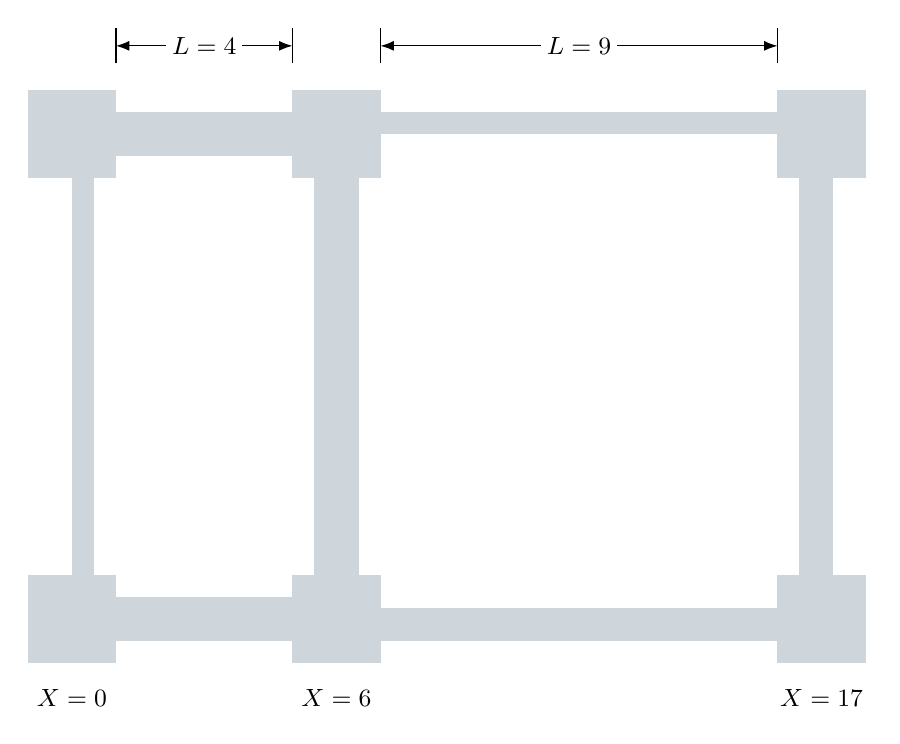
\begin{tikzpicture}[x=.56cm,y=.56cm]
 \foreach \x in {0,6,17}{\foreach \y in {0,11}{
   \fill[domainblue!24] (\x-1,\y-1) rectangle (\x+1,\y+1);}}
 \fill[domainblue!24] (1,-.5) rectangle (5,.5);
 \fill[domainblue!24] (1,10.5) rectangle (5,11.5);
 \fill[domainblue!24] (7,-.5) rectangle (16,.25);
 \fill[domainblue!24] (7,11) rectangle (16,11.5);
 \fill[domainblue!24] (0,1) rectangle (.5,10);
 \fill[domainblue!24] (5.5,1) rectangle (6.5,10);
 \fill[domainblue!24] (16.5,1) rectangle (17.25,10);
 \foreach \x in {0,6,17}{
   \node[font=\small] at (\x,-1.8) {$X=\x$};}
 \draw[thin,<->,>=Latex] (1,13)--(5,13);
 \node[font=\small,fill=white,inner sep=2pt] at (3,13) {$L=4$};
 \draw[thin,<->,>=Latex] (7,13)--(16,13);
 \node[font=\small,fill=white,inner sep=2pt] at (11.5,13) {$L=9$};
 \draw[thin] (1,12.6)--(1,13.4) (5,12.6)--(5,13.4)
              (7,12.6)--(7,13.4) (16,12.6)--(16,13.4);
\end{tikzpicture}
\caption{An actual nonuniform network, with side-two room centers
at $\{0,6,17\}\times\{0,11\}$. The left horizontal passages have
$(L,w,\eta)=(4,1,0)$. The right passages have $(9,3/4,-1/8)$ below
and $(9,1/2,1/4)$ above. The vertical passages, from left to right,
have $(9,1/2,1/4)$, $(9,1,0)$, and $(9,3/4,-1/8)$.
Horizontal offsets are measured upwards and vertical offsets to
the right. All lengths and widths are drawn at the same scale.}
\label{fig:nonuniform}
\end{figure}

For example, on a grid of spacing eleven, every selected corridor has
length nine. Its width may be chosen independently in $[4/9,1]$.
A width-$1/2$ corridor may be displaced by any amount up to $1/4$
from the face center. After scaling rooms back to side one, this gives
width $1/4$, length $9/2$, and displacement up to $1/8$. The resulting
families allow degree-four branching and arbitrary finite selected-edge
patterns as well as these continuous geometric parameters.

The allowed range also contains passages of fixed area and arbitrarily
small width: take $0<w\le4/9$ and $L=4/w$. Then $L\ge9$ and $Lw=4$,
the area of a base corridor. Such passages can be realized by choosing
the corresponding coordinate gap $2+4/w$; different bands may have
different gaps. This describes a genuine parameter family, not an
assertion that arbitrary prescribed edge lengths satisfy the closure
constraints of every cyclic drawing.

The restrictions in \eqref{nu:edge-ranges} and
\eqref{nu:port-envelope} are part of the result. In particular, the
argument gives neither arbitrary width perturbations at length four
nor displaced full-width ports. It uses the full physical corridor
areas and their counting differences to pay the chamber comparison;
it does not assume monotonicity
of the corridor count divided by area.

\section{Independent port displacements and corridor subdivision}
\label{sec:chains}

The compact network result keeps each port centered. A second cell
inequality permits an independent displacement at each end of a passage.
The two applications use the same distinction: symmetry may simplify
the comparison problem even when the physical domain has no symmetry.

\subsection{An offset-chain family}

Let $B=(0,1)\times(0,2)$. Give it Neumann conditions on the two
segments $\{0,1\}\times(1/3,5/3)$ and Dirichlet conditions on the
rest of the boundary. Continue to write $R$ for the $4$-by-$1$
rectangle with Neumann ends and Dirichlet long sides. We will prove
\begin{equation}\label{ch:module}
 N_B(E)+N_R(E)\le\frac{6E}{4\pi}\qquad(E>0).
\end{equation}
The enlarged windows of $B$ contain every unit-length interval
whose lower endpoint lies in $[1/3,2/3]$.

For $n\ge1$, choose real numbers $c_j,a_j$, $0\le j<n$, with
\begin{equation}\label{ch:offsets}
 \frac13\le a_j-c_j\le\frac23\quad(0\le j<n),\qquad
 \frac13\le a_j-c_{j+1}\le\frac23\quad(0\le j<n-1).
\end{equation}
Define the open chain as the interior of
\begin{equation}\label{ch:geometry}
 \bigcup_{j=0}^{n-1}\left(
 [5j,5j+1]\times[c_j,c_j+2]
 \ \cup\ [5j+1,5j+5]\times[a_j,a_j+1]\right).
\end{equation}
Its area is $6n$. Cutting each actual interface and enlarging the
allowed chamber traces to those of $B$ gives
\[
 N_\Om(E)\le n\bigl(N_B(E)+N_R(E)\bigr)
 \le\frac{6nE}{4\pi}.
\]
At the two physical ends a Dirichlet boundary is only relaxed,
never replaced by a stronger boundary condition. Thus
\eqref{ch:module} proves P\'olya's inequality for every chain
\eqref{ch:geometry}, including all endpoint equalities in
\eqref{ch:offsets}.

The incoming and outgoing offsets at a chamber need not be equal.
Specifying them successively determines the vertical drift of the
chambers; the disjoint horizontal slabs prevent unintended
intersections. No bound on the number of chambers is used.

The one-chamber members also admit a direct inheritance argument.
After translation such a member is
\[
 S_\delta=\operatorname{int}\bigl(
 [0,1]\times[0,2]\ \cup\ [1,5]\times[\delta,\delta+1]\bigr),
 \qquad\frac13\le\delta\le\frac23.
\]
Its image under $(x,y)\mapsto(6-x,y+1)$ has disjoint interior.
Together the two copies form a parent whose vertical sections,
away from the joining lines, are $[0,2]$ for $0<x<1$,
$[\delta,\delta+2]$ for $1<x<5$, and $[1,3]$ for $5<x<6$.
The vertical translates of this parent by $2\mathbb Z$ tile a
strip, so congruent-subtile inheritance also proves P\'olya's
inequality for $S_\delta$; see \cite{FLPS,JiangLin}. The cell
proof below treats the entire independently displaced chain family.

\begin{figure}[tb]
\centering
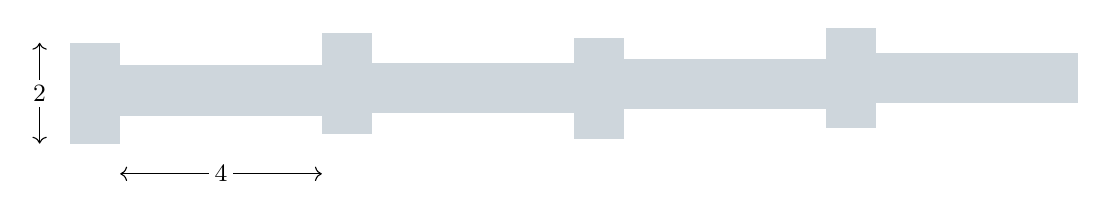
\begin{tikzpicture}[x=.64cm,y=.64cm]
 \foreach \j/\c/\a in {0/0/.55,1/.2/.6,2/.1/.68,3/.3/.8}{
  \fill[domainblue!24] ({5*\j},\c) rectangle ({5*\j+1},{\c+2});
  \fill[domainblue!24] ({5*\j+1},\a) rectangle ({5*\j+5},{\a+1});}
 \draw[<->,thin] (1,-.6)--(5,-.6);
 \node[fill=white,font=\small,inner sep=2pt] at (3,-.6) {$4$};
 \draw[<->,thin] (-.6,0)--(-.6,2);
 \node[fill=white,font=\small,inner sep=2pt] at (-.6,1) {$2$};
\end{tikzpicture}
\caption{An exact offset-chain geometry with four chambers. The
chamber bottoms are $0,1/5,1/10,3/10$ and passage bottoms are
$11/20,3/5,17/25,4/5$. All incoming and outgoing offsets satisfy
\eqref{ch:offsets}. The drawing uses equal horizontal and vertical
units; neither passage lengths nor vertical displacements are exaggerated.}
\label{fig:chain}
\end{figure}

\subsection{The two boundary corrections}

Relax both vertical faces of $B$ completely to Neumann and call
the resulting problem $B_0$. At $E=\pi^2r^2$ its spectrum and
that of $R$ give the exact sum
\begin{equation}\label{ch:coarse}
 \begin{split}
 Q_0(r)&=N_{B_0}(\pi^2r^2)+N_R(\pi^2r^2)\\
 &=\lfloor2r\rfloor+\lfloor r\rfloor
 +\sum_{m=1}^{\lfloor r\rfloor}
 \left(\left\lfloor2\sqrt{r^2-m^2}\right\rfloor
       +\left\lfloor4\sqrt{r^2-m^2}\right\rfloor\right).
 \end{split}
\end{equation}
In units of $\pi^2$, the individual levels are
$m^2/4+n^2$, $m\ge1,n\ge0$, for $B_0$, and
$m^2+n^2/16$, $m\ge1,n\ge0$, for $R$.
At $r^2=5/4$ the sum is six, exceeding $15\pi/8$;
at $r^2=5$ it is twenty-four, exceeding $15\pi/2$.

The problem $B$ is invariant under reflection in both midlines.
Write a minus sign for odd parity and a plus sign for even parity.
In the $(-,+)$ sector, use distances from the midlines as
coordinates on $Q=(0,1/2)\times(0,1)$. The comparison has
Dirichlet condition at $x=0$ and $y=1$, and Neumann condition
at $x=1/2$ and $y=0$. The actual problem adds Dirichlet
condition on $\{1/2\}\times(2/3,1)$. Its normalized ground
mode and data for \eqref{bd:scalar-lift} are
\[
 \phi_1=\sqrt8\sin(\pi x)\cos(\pi y/2),\qquad
 \lambda_0=5\pi^2/4,\quad \Delta=2\pi^2,\quad
 g_1=\frac43-\frac{2\sqrt3}{\pi}.
\]
The trace formula follows by integrating $8\cos^2(\pi y/2)$
over $(2/3,1)$. The resulting bound is
\begin{equation}\label{ch:first-lift}
 \lambda_1^{-,+}(B)
 \ge\frac{5\pi^2}{4}
   +\frac{2\pi^2g_1}{g_1+\pi\sqrt{13}}
 >\frac{41\pi^2}{32}.
\end{equation}
Indeed $g_1>16/75$, using $\pi>25/8$ and $\sqrt3<7/4$;
therefore $63g_1>336/25>88/7>\pi\sqrt{13}$, which is
the required strict inequality.

In the $(-,-)$ sector the quarter comparison has Dirichlet
condition at $x=0$ and $y=0,1$, and Neumann condition at
$x=1/2$. Its first three levels are $2\pi^2,5\pi^2,10\pi^2$.
Apply \eqref{bd:scalar-lift} at the second, simple level,
imposing orthogonality to the comparison ground mode. The data are
\[
 \phi_2=\sqrt8\sin(\pi x)\sin(2\pi y),\qquad
 \lambda_0=5\pi^2,\quad\Delta=5\pi^2,\quad
 g_2=\frac43+\frac{\sqrt3}{2\pi}.
\]
Thus
\begin{equation}\label{ch:second-lift}
 \lambda_2^{-,-}(B)
 \ge5\pi^2+\frac{5\pi^2g_2}{g_2+2\pi\sqrt{10}}
 >\frac{21\pi^2}{4}.
\end{equation}
For the last comparison, $19g_2>76/3>176/7>
2\pi\sqrt{10}$. Multiplicity of the next level causes no
problem: the gap above the simple second level is still $5\pi^2$.

All other levels remain bounded below by their comparison levels.
Consequently $N_B+N_R$ is bounded by $Q_0-1$ when
\begin{equation}\label{ch:corrections}
 40\le32r^2<41\qquad\text{or}\qquad160\le32r^2<168,
\end{equation}
and by $Q_0$ elsewhere. The upper endpoints are deliberately
excluded from the correction, though the strict spectral bounds
would allow them. Their upper-count jumps will be tested directly.

\subsection{A short explicit tail for the chain}

Put $f_r(y)=\sqrt{r^2-y^2}$, $M=\lfloor r\rfloor$ and $s=r-M$.
Concavity, the trapezoidal inequality, and the chord on the final
interval give
\begin{equation}\label{ch:circle-sum}
 \begin{split}
 \sum_{m=1}^M f_r(m)
 &\le\frac{\pi r^2}{4}-\frac r2+
       \frac{f_r(M)}2-\int_M^r f_r(y)\dd y\\
 &\le\frac{\pi r^2}{4}-\frac r2+
       \frac{(1-s)\sqrt{2rs}}2
 \le\frac{\pi r^2}{4}-\frac r2+
       \frac{\sqrt{2r}}{3\sqrt3}.
 \end{split}
\end{equation}
Define
\[
 F(r)=\sum_{m=1}^M\left(\{2f_r(m)\}+\{4f_r(m)\}\right).
\]
Bounding the zero-frequency rows in \eqref{ch:coarse} by $3r$
and using \eqref{ch:circle-sum} yields
\begin{equation}\label{ch:tail-excess}
 Q_0(r)\le\frac{3\pi r^2}{2}+2\sqrt{\frac23}\sqrt r-F(r).
\end{equation}
A two-row version of the fractional-block argument suffices here.
For $a=2,4$, the magnitude of the derivative of $af_r$ at $y=rx$
is $ax/\sqrt{1-x^2}$. On each interval $[p/1000,q/1000]$
in the following table it lies in $[j+1/4,j+3/4]$.
\begin{table}[tb]
\centering
\begin{tabular}{@{}rcc@{}}
\toprule
$j$&$(p,q)$ for $a=2$&$(p,q)$ for $a=4$\\\midrule
0&(125,351)&(63,184)\\
1&(530,658)&(299,400)\\
2&(748,808)&(491,566)\\
3&(852,882)&(631,683)\\
4&(905,921)&(729,764)\\
5&(935,944)&(796,820)\\
6&(953,958)&(843,860)\\
7&(964,968)&(876,888)\\
8&(972,974)&(900,909)\\
9&(978,979)&(918,925)\\\bottomrule
\end{tabular}
\caption{Rational derivative windows for the chain count.
The intervals are disjoint within each column and their total
length over both columns is $934/1000$.}
\label{ch:windows}
\end{table}
These assertions are the integer inequalities
\begin{equation}\label{ch:window-integers}
 \begin{split}
 [16a^2+(4j+1)^2]p^2&\ge(4j+1)^2\,10^6,\\
 [16a^2+(4j+3)^2]q^2&\le(4j+3)^2\,10^6.
 \end{split}
\end{equation}
An interval of length $w$ in the $x$ variable contains at least
$rw/2-1$ disjoint pairs of consecutive integer rows after scaling
by $r$. In each pair the two values of $af_r$ differ by a number
whose fractional part lies in $[1/4,3/4]$. Their two fractional
parts therefore sum to at least $1/4$: for a difference with
fractional part $d$, the sum is at least $\min(d,1-d)$.
Summing the twenty disjoint-window contributions gives
\begin{equation}\label{ch:loss}
 F(r)\ge\frac{934}{8000}r-5.
\end{equation}
For $r\ge300$, use $2\sqrt{2/3}<5/3$, $\sqrt r\le r/17$
and $5\le r/60$. Since
$934/8000-1/60>5/51$, \eqref{ch:tail-excess} proves
\begin{equation}\label{ch:tail}
 Q_0(r)\le\frac{3\pi r^2}{2}\qquad(r\ge300).
\end{equation}

\subsection{The remaining finite interval}

Use $X=32r^2$ for this cell. All comparison events below $r=300$
are the integers
\begin{equation}\label{ch:events}
 \begin{aligned}
 X&=8m^2+32n^2,&1\le m\le600,&\quad0\le n\le300,\\
 X&=32m^2+2n^2,&1\le m\le300,&\quad0\le n\le1200,
 \end{aligned}
\end{equation}
retaining only $X\le2{,}880{,}000$. These bounds are exhaustive
by positivity of the summands. Add the artificial events $X=41,168$.
At each event form the complete inclusive comparison count and
subtract one exactly in the intervals \eqref{ch:corrections}.
Call the resulting upper count $U(X)$. The finite integer certificate is
\begin{equation}\label{ch:integer}
 6784\,U(X)\le999X.
\end{equation}
It suffices because $\pi>333/106$. Direct enumeration by the
algorithm in Appendix~\ref{app:certificates} gives $135{,}424$
actual event levels and $135{,}426$ levels after adding the resets.
The minimum of $999X-6784U(X)$ is $255$, attained at $X=41$,
where $U(X)=6$. The comparison count at the cutoff is $423{,}767$.
The same verifier checks every inequality in
\eqref{ch:window-integers} and the total window length.

Between successive events $U$ is constant and the area term
increases; before the first event the count is zero. Thus the
finite certificate proves \eqref{ch:module} through $r=300$.
Together with \eqref{ch:tail} it proves \eqref{ch:module} for
every energy, completing the offset-chain assertion.

One related boundary convention is useful. Replace the final
full passage by two terminal $2$-by-$1$ passages, one at each
end of a chain with $n$ chambers and $n-1$ full passages. Each
terminal passage has a physical Dirichlet end and a Neumann cut
at its chamber. For a transverse row with
$s=\sqrt{E/\pi^2-m^2}$, their combined count is
$2\lfloor2s+1/2\rfloor\le\lfloor4s\rfloor+1$.
Indeed, writing $2s=j+t$ with $0\le t<1$ verifies this in the
two cases $t<1/2$ and $t\ge1/2$. The total terminal count is
therefore at most that of one full passage. The area remains
$6n$, so the all-energy bound holds for this two-ended variant too.

\subsection{Redistributing an actual corridor budget}

The same local inequality permits a useful geometric dissection.
If $w_1,\ldots,w_s>0$ and $\sum_iw_i=1$, imposing Dirichlet
conditions along longitudinal lines in $R$ gives
\begin{equation}\label{ch:width-split}
 \sum_{i=1}^s N_{R(4,w_i)}(E)\le N_R(E).
\end{equation}
Here $R(L,w)$ denotes a rectangle of length $L$ and width $w$,
with Neumann ends and Dirichlet long sides. Extension by zero
from the strips gives an isometric embedding of their direct-sum
form domain into that of $R$, proving the direction of
\eqref{ch:width-split}. In contrast, cutting a long passage into
$k$ length-four pieces with Neumann cuts gives
\begin{equation}\label{ch:length-split}
 N_{R(4k,w)}(E)\le kN_{R(4,w)}(E).
\end{equation}
Both comparisons preserve actual area.

Suppose a finite physical assembly has $n$ copies of the chamber
underlying $B$, with every interface on its permitted windows,
and rectangular passages that can be cut into length-four pieces.
Assume those pieces can be grouped into $n$ groups whose widths
each sum to one. All other boundary segments are physical
Dirichlet boundary, and piece interiors are disjoint. Cutting
the assembly, applying \eqref{ch:width-split} in each group,
and then \eqref{ch:module} proves
\[
 \abs\Om=6n,\qquad N_\Om(E)\le\frac{6nE}{4\pi}.
\]
This assertion concerns an actual embedded assembly; it does
not assert that every abstract graph admits such an embedding.
The width grouping is also substantive: a total sum equal to
$n$ does not by itself replace the required partition into
$n$ unit-width groups. These explicit conditions keep the
comparison tied to the physical passage area.

\section{What the retained boundary controls}\label{sec:limits}

The proofs isolate a local distinction. Fully separated
rectangular cells make all frequencies accessible to exact
counting, but they can have too many low modes. Retaining the
physical Dirichlet segments removes precisely the modes needed
in the present geometries. The correction is independent of
the size of the assembled graph, which is why arbitrary finite
combinatorial complexity causes no accumulation of error.

It is important that some Dirichlet boundary remains. The
following direct example explains why independent-cell
estimates cannot be uniform over unrestricted port widths.
Take a unit-square chamber with four centered Neumann ports
of width $w=1-2\varepsilon$, retaining Dirichlet condition on
the corner segments. Put $R_0=1/4$ and $0<\varepsilon<R_0$.
At each corner choose a function that is zero within distance
$\varepsilon$, equals
\[
 \frac{\log(r/\varepsilon)}{\log(R_0/\varepsilon)}
 \quad\text{for }\varepsilon<r<R_0,
\]
and is one outside the four quarter-disks of radius $R_0$.
This is an admissible $H^1$ trial function for the mixed chamber.
The four quarter-annuli have total energy
$2\pi/\log(R_0/\varepsilon)$, and its squared norm is at least
$1-\pi/16$. Consequently
\begin{equation}\label{eq:wide-port-limit}
 \lambda_1(C_w)\le
 \frac{2\pi}{(1-\pi/16)\log(R_0/\varepsilon)}\longrightarrow0.
\end{equation}
If the four passages have length two, their half-shares assign
area $1+4w\le5$ to the chamber. Their first transverse level
is $\pi^2/w^2$. For small enough $\varepsilon$ one can choose
an energy below both $4\pi/5$ and $\pi^2/w^2$ but above the
upper bound in \eqref{eq:wide-port-limit}. The separated
chamber count is then at least one, the passage count is zero,
and the proposed local area bound is strictly less than one.
Thus that separated comparison really fails. The conclusion
concerns the independent cells, not the coupled Dirichlet
domain, whose matching conditions were discarded.

At the fixed dimensions of the main construction, all six
chamber types are covered, including the fully branching
four-port junction. The compact and chain comparisons, together with
the explicit nonuniform extension, show how sharp global counts can
follow from quantitative boundary corrections, complete tail control,
and exact accounting at the actual interfaces.
Allowing unrestricted passage widths or lengths requires new local estimates
or a comparison that retains more of the coupling at the
interfaces. The all-eigenvalue conclusions proved here do
not require such an extension.

\appendix

\section{Exact arithmetic certificates}
\label{app:certificates}

This appendix specifies the scalar arithmetic, block integrals, and
degree-at-most-three and chain event computations used in the proof. All
loops have explicit finite bounds, all comparisons use integers or
rationals, and all eigenvalue multiplicities are retained.

\subsection{Rational constants}

For a positive integer $q$, let
\[
 S_N(q)=\sum_{j=0}^{N-1}\frac{(-1)^j}{(2j+1)q^{2j+1}}.
\]
The alternating-series bound and Machin's identity give
\[
 \ell=16S_{12}(5)-4S_5(239)<\pi
 <16S_{13}(5)-4S_4(239)=u.
\]
The identity follows by applying the tangent addition formula to
$4\arctan(1/5)-\arctan(1/239)$; its tangent is one and its angle lies
in $(0,\pi/2)$. Direct rational comparison gives
\begin{equation}
 \ell>\frac{103993}{33102}>\frac{333}{106}>\frac{25}{8},
 \qquad u<\frac{22}{7},\qquad u^2<10.
 \label{app:pi-bounds}
\end{equation}
Thus every use of $\pi$ in the finite checks can be replaced by the
displayed rational bounds. Fractions are compared by cross multiplication
of their positive denominators.

For completeness, the strict margins in the degree-three boundary
calculation reduce to
\[
 \begin{split}
 A_0&=\left(\frac{64}{625}\right)^2\frac{32}{15}
       +\frac{64}{625}\frac{23}{7}\frac3{20}
       =\frac{2987504}{41015625},\\
 A_0&<\frac{73}{1000},\\
 \frac1{12}+\frac{73}{1000}&=\frac{469}{3000},\\
 2\left(\frac{73}{1000}+\frac38\frac{64}{625}\right)
 &=\frac{557}{2500},\\
 4\frac{469}{3000}+\frac{557}{2500}
 &=\frac{6361}{7500},\qquad
 \frac{17}{20}-\frac{6361}{7500}=\frac7{3750}>0.
 \end{split}
\]
These give the matrix majorant in \eqref{bd:gram-majorant}. The strict
endpoint in \eqref{bd:double-lift} follows from $\pi^2<10$ and
\[
 \frac{20}{17\cdot10+20}=\frac2{19},\qquad
 \frac{25}{16}+\frac2{19}=\frac{507}{304},\qquad
 \frac{507}{304}-\frac53=\frac1{912},\quad
 \frac53-\frac{53}{32}=\frac1{96}.
\]
The associated endpoint comparison has margin
\[
 \frac{53}{32}\frac{333}{106}-\frac{26}{5}=\frac1{320}>0.
\]
The first six even-sector numerators, in units of $\pi^2/16$, are
$1,9,17,25,25,41$; the first three odd-sector numerators are $5,13,29$.
They are obtained from
$16m^2+(2n+1)^2$ and $4(2m+1)^2+(2n+1)^2$, respectively. The ranges
$0\le m\le2$, $0\le n\le3$ contain these initial levels and every
level at or below $53/2$; positivity of the square terms excludes all
other indices. This also checks the multiplicity used in the cluster
argument.

The simpler boundary comparisons use
\[
 1+\frac{22}{7}\,4<64,\qquad
 \frac43-\frac{2(7/4)}{25/8}=\frac{16}{75},\qquad
 63\frac{16}{75}>\frac{88}{7},\qquad
 19\frac43>\frac{176}{7},
\]
together with $\sqrt3<7/4$, $\sqrt{13}<4$, and $\sqrt{10}<4$.
They verify the opposite-port and both offset-chain lift thresholds.

\subsection{The fractional-block integral lower sums}

Set $L=8192$ and $D=10^9$ for $(a,K,G)=(1,6,2)$ or $(4,4,4)$.
Set $L=32768$ and $D=10^{12}$ for $(a,K,G)=(1,13,3)$ or $(4,7,8)$.
For each choice and every integer $0\le j\le GL$, define
\[
 b_j=\operatorname{isqrt}\left(
      \left\lfloor\frac{D^2j^2}{a^2L^2+j^2}\right\rfloor\right),
\]
where $\operatorname{isqrt}(n)=\lfloor\sqrt n\rfloor$ for a
nonnegative integer $n$. Thus
\[
 \frac{b_j}{D}\le\frac{j}{\sqrt{a^2L^2+j^2}}
                    <\frac{b_j+1}{D}.
\]
For $0\le j<GL$, let
\[
 \begin{split}
 m_j&=\min_{0\le s<K}\sum_{k=0}^{K-1}
                   ((s-k)j\bmod L),\\
 h_j&=\max\{0,m_j-C_K\},\qquad
 w_j=\max\{0,b_{j+1}-b_j-1\}.
 \end{split}
\]
The residue in the first line is the unique integer in
$\{0,\ldots,L-1\}$. Formula~\eqref{eq:block-minimum} gives
$M_K(j/L)=m_j/L$, and \eqref{eq:block-lipschitz} bounds the integrand
below by $h_j/L$ throughout the slope interval $[j/L,(j+1)/L]$.
Under the increasing substitution $x=s/\sqrt{a^2+s^2}$, that interval
has $x$-width at least $w_j/D$. Consequently
\begin{equation}
 A(a,K,G)\ge\frac1{KLD}\sum_{j=0}^{GL-1}h_jw_j.
 \label{app:integral-sum}
\end{equation}
The integer algorithm is completely specified by
\begin{verbatim}
parameters = [(1,6,2,8192,10**9), (4,4,4,8192,10**9),
              (1,13,3,32768,10**12), (4,7,8,32768,10**12)]
for (a,K,G,L,D) in parameters:
    C = K*(K-1)//2
    total = 0
    b = 0
    for j in range(G*L):
        t = j+1
        next_b = isqrt((D*D*t*t)//(a*a*L*L+t*t))
        m = min(sum(((s-k)*j) % L for k in range(K))
                for s in range(K))
        # Lower height times lower width, both nonnegative.
        total += max(0,m-C)*max(0,next_b-b-1)
        b = next_b
    return Fraction(total,K*L*D)
\end{verbatim}
Here ``return'' means recording the value for the current triple. In the
listed order, the integer totals are
\[
 \begin{gathered}
 12900023357295,\qquad5549929653480,\\
 150528062155176292,\qquad64044999196269018.
 \end{gathered}
\]
After cancellation, \eqref{app:integral-sum} gives exactly the fractions
in \eqref{eq:block-integrals} and \eqref{eq:degree-four-integrals}.
Their comparisons to $13/50$, $169/1000$, $353/1000$, and $279/1000$
are strict rational comparisons. Neither square root is evaluated
approximately.

The block errors in \eqref{eq:fractional-block} are, respectively,
\[
 \frac{6^2\cdot2}{8}+\frac62=12,\qquad
 \frac{4^2\cdot4}{8}+\frac42=10,\qquad
 \frac{13^2\cdot3}{8}+\frac{13}{2}=\frac{559}{8},\qquad
 \frac{7^2\cdot8}{8}+\frac72=\frac{105}{2}.
\]
The remaining degree-at-most-three tail arithmetic is
\[
 \frac2{27}<\frac9{121},\qquad 2<\frac{100}{49},\qquad
 \frac3{11}\left(\frac{10}{7}+6\right)=\frac{156}{77},
 \qquad 800<29^2,
\]
and
\[
 -\frac{547}{2000}\,800+\frac{156}{77}\,29+28
 =-\frac{50838}{385}<0.
\]
For degree four,
\[
 \begin{gathered}
 2\frac{353}{1000}+2\frac{279}{1000}-1=\frac{33}{125},\qquad
 \frac3{11}\left(\frac{10}{7}+8\right)=\frac{18}{7},\\
 1+\frac{559}{8}+2\frac{105}{2}=\frac{1407}{8},\qquad
 -\frac{33}{125}\,1024+\frac{18}{7}\,32+\frac{1407}{8}
 =-\frac{85227}{7000}<0.
 \end{gathered}
\]

\subsection{Every compact-cell event}

Set $Q=10240000$. For each of the five triples
\[
 (s_x,s_y,d)=(2,2,0),(2,1,1),(2,0,2),(1,1,2),(1,0,3),
\]
make zero-filled integer arrays $H[0],\ldots,H[Q]$ and
$R[0],\ldots,R[Q]$. A shared array $R$ may be reused for all five
types. The following loops generate their complete multiplicities:
\begin{verbatim}
# Chamber: x = s_x mod 2, y = s_y mod 2, with these minima.
for x in range(s_x,isqrt(Q)+1,2):
    for y in range(s_y,isqrt(Q-x*x)+1,2):
        H[x*x+y*y] += 1
# Corridor: its transverse index y is positive and divisible by 4.
for x in range(0,isqrt(Q)+1):
    for y in range(4,isqrt(Q-x*x)+1,4):
        R[x*x+y*y] += 1
\end{verbatim}
The first loop has step two even when $s_x=2$ or $s_y=2$, so zero
frequencies are present only in the NN coordinates. Each pair of
nonnegative squares satisfying the stated threshold lies in exactly
one iteration. Thus the bounds are exhaustive.

Set $h=r=0$. For $p=0,1,\ldots,Q$, first replace
$h$ by $h+H[p]$ and $r$ by $r+R[p]$. If $H[p]+R[p]>0$, use
$c=c_S(p)$ from \eqref{eq:compact-corrections} with $N_H=h$ and check
\begin{verbatim}
# Count all eigenvalues equal to p before making the comparison.
require(h >= c)
U = 2*(h-c) + d*r
require(103993*(2+d)*p - 16*33102*U >= 0)
\end{verbatim}
All quantities are integers. Tracking the number of such checks and
their minimum margin produces the actual-event table in
Section~\ref{sec:finite-closure}. Checking the same margin with $c=0$
produces exactly the four deficient events reported there.

Also record $(h,r)$ after $p=2,20,26$. At each applicable reset
$q=8/3,41/2,53/2$, use the recorded counts after $p=\lfloor q\rfloor$,
evaluate $c_S(q)=0$, and perform the same comparison with $q$ in place
of $p$, now as a rational. The resulting four margins are precisely
those in the reset table. This extra instruction is necessary because
the corrected upper count can jump when a correction ceases even though
the separated spectrum has no eigenvalue there. All starts of corrections
are already actual events. The count at $Q$ is checked because the
corridor pair $(x,y)=(0,3200)$ has this event.

The released implementation uses compact arrays only for the individual
multiplicities. Their entries cannot exceed the total number of pairs in
the enclosing index rectangles, which is less than $3201^2<2^{32}$.
Every cumulative count, multiplication, and margin comparison uses
arbitrary-precision integers. Thus fixed-width overflow cannot affect an
acceptance decision.

\subsection{Every offset-chain event}

Use the separate coordinate $X=32r^2$ from the offset-chain calculation,
and set $Q_c=2880000=32\cdot300^2$. Initialize an integer array
$J[0],\ldots,J[Q_c]$ to zero and execute
\begin{verbatim}
# Separated chamber, including its zero longitudinal mode.
for m in range(1,isqrt(Q_c//8)+1):
    base = 8*m*m
    for n in range(0,isqrt((Q_c-base)//32)+1):
        J[base+32*n*n] += 1
# Corridor, including its zero longitudinal mode.
for m in range(1,isqrt(Q_c//32)+1):
    base = 32*m*m
    for n in range(0,isqrt((Q_c-base)//2)+1):
        J[base+2*n*n] += 1
\end{verbatim}
These ranges are exactly the nonnegative solutions of the two spectral
inequalities. The chamber indices satisfy $1\le m\le600$,
$0\le n\le300$; the corridor indices satisfy $1\le m\le300$,
$0\le n\le1200$. Initialize $b=0$, and for each integer
$x=0,\ldots,Q_c$ first add $J[x]$ to $b$. At every $x$ with $J[x]>0$,
and also at $x=41,168$, execute
\begin{verbatim}
# Equality at the left endpoints is included; resets are excluded.
c = int((40 <= x < 41) or (160 <= x < 168))
require(b >= c)
require(999*x - 6784*(b-c) >= 0)
\end{verbatim}
This is the rational comparison \eqref{ch:integer}. There are $135424$
actual jump levels and $135426$ checked levels after the two resets
are added. The total coarse multiplicity at $Q_c$ is $423767$.
The only deficient levels before the correction are $X=40,160$.
The minimum corrected margin is $255$ at $X=41$, with upper count six;
the other reset, $X=168$, has upper count twenty-four and margin $5016$.
The endpoint $Q_c$ is itself an actual event and is included.

For the analytic chain tail, the twenty intervals in
Table~\ref{ch:windows} are checked without square roots. For its row
$(a,j,p,q)$, check
\[
 [16a^2+(4j+1)^2]p^2\ge(4j+1)^2\,10^6,
 \qquad
 [16a^2+(4j+3)^2]q^2\le(4j+3)^2\,10^6,
\]
together with the listed order and disjointness of the intervals for
each fixed $a$. Their width numerators sum to $934$. The final tail
comparison has the exact positive margin
\[
 \frac{934}{8000}-\frac1{60}-\frac5{51}
 =\frac{139}{68000}>0.
\]
As a second arithmetic check, the affine lower bound at $r=300$ equals
$1201/40$, whose square exceeds $800$. For
$s=934/8000$, one also has $2s(1201/40)>8/3$, so the difference
$(sr-5)^2-8r/3$ is increasing for $r\ge300$. This verifies the same
tail endpoint and monotonicity used in the text.

\section{Exact arithmetic for the four-port chamber}
\label{df:appendix}

This appendix specifies the finite certificates used in
Section~\ref{sec:degree-four}. Every comparison uses integers or
rational intervals. The spectral complement outside each finite
square is supplied by \eqref{df:complete-tail}; no numerical
eigenvalue approximation enters the argument.

\subsection{Interval matrices}

Let
\[
 A=2^{48},\qquad
 S_N(q)=\sum_{j=0}^{N-1}\frac{(-1)^j}{(2j+1)q^{2j+1}},
\]
and take the rational Machin bounds
\[
 \ell=16S_{12}(5)-4S_5(239),\qquad
 u=16S_{13}(5)-4S_4(239).
\]
The alternating-series argument in
Appendix~\ref{app:certificates} gives
$103993/33102<\ell<\pi<u<22/7$.
Represent a closed interval by its integer endpoints $[L,U]/A$.
For a rational $x=p/q$, $q>0$, use
\[
 \operatorname{enc}(x)=
 \left[\left\lfloor\frac{Ap}{q}\right\rfloor,
       \left\lceil\frac{Ap}{q}\right\rceil\right]/A.
\]
Addition and negation operate exactly on endpoints. For a product,
form all four products of integer endpoints, divide their minimum
and maximum by $A$, and round respectively down and up. For division
by a positive interval, form all four ratios $Ax/y$ of integer
endpoints and round their minimum and maximum outwards. Each
resulting interval still has denominator $A$. Thus every individual
operation encloses the corresponding exact operation, even when
its two arguments are dependent.

Enclose $1/\pi$ by rounding $1/u$ down and $1/\ell$ up. Evaluate
\eqref{df:J} as a rational constant plus a rational multiple of this
interval. The sine of an even integer multiple of $\pi/4$ is obtained
from the repeating integer list $0,1,0,-1$, and the zero-frequency
term contributes $1/2$ to $J$. Opposite-parity entries are exactly
zero. Construct $D$, $W$, and $S_e^{(128)}$ from
\eqref{df:coupling} and the definitions in
Section~\ref{sec:degree-four}, using interval operations throughout.
In particular, the denominator for a high pair $(m,n)$ is
$d_md_n((m^2+n^2)/4-e)$, with no omission of zero-index norm factors.

Here is complete loop-level pseudocode for a row $(P_*,s)$ of the
table. A block vector is stored as a list of triples $(a,b,c)$
meaning $\sum c\Psi_{ab}$.
\begin{verbatim}
e = Pstar/16
low = [(m,n) in increasing m, then increasing n:
       m,n >= 0 and m*m+n*n < 4*e]
block = [[(m,n,1)] for (m,n) in low if m*m+n*n >= s]
if Pstar == 41/2:
    block = [[(0,2,1),(2,0,1)], [(1,2,1)], [(2,1,1)]]
k = len(block)
B(i,m,n) = sum over (a,b,c) in block[i] of
    c*((1+(-1)**(a+m))*J(b,n)+(1+(-1)**(b+n))*J(a,m))
D[i,j] = sum(c*B(i,a,b) for (a,b,c) in block[j])
q[j] = (a*a+b*b)/4 for any (a,b,c) in block[j]
norm[j] = sum(c*c*d[a]*d[b] for (a,b,c) in block[j])
W[j] = (e-q[j])*norm[j]
S = zero k by k matrix
for m = 0,...,128:
    for n = 0,...,128:
        if (m*m+n*n)/4 > e:
            v = [B(i,m,n) for i = 0,...,k-1]
            den = d[m]*d[n]*((m*m+n*n)/4-e)
            S[i,j] += v[i]*v[j]/den for 0 <= i <= j < k
mirror the upper triangle of S
T[i,j] = sum(D[i,t]*D[j,t]/W[t] for t = 0,...,k-1)
         - S[i,j] - D[i,j]/3
for t = 0,...,k-1:
    pivot = T[t,t]
    check lower_endpoint(pivot) > 3/4
    for i = t+1,...,k-1:
        for j = i,...,k-1:
            T[i,j] = T[j,i] = T[i,j]-T[i,t]*T[j,t]/pivot
check len(low)-k equals the tabulated cap
\end{verbatim}
All list bounds are finite: each index in \texttt{low} is at most
$\lfloor\sqrt{4e}\rfloor$. The construction also checks that no
Neumann mode equals $e$, that each block column has one energy,
and that every division has a strictly positive denominator interval.
The loops use exactly the ordering displayed above. Interval
symmetric elimination encloses every exact Schur complement by
induction; positive pivots therefore certify positive definiteness
of the exact matrix. The common smallest pivot lower endpoint is
\eqref{df:pivot-margin}. This proves all 28 finite-matrix comparisons
by an explicitly reproducible rational computation.

The uniform tail constant used here needs only the rational check
\[
 4\left[
 \frac4{128\bigl(1-(3413/8)/129^2\bigr)}
 +\frac2{129^2-3413/8}+\frac{2(22/7)}{127}\right]
 =\frac{7536117}{23063327}<\frac13.
\]
Since $129^2-3413/8>127^2$, this dominates
$\varepsilon(128,e)$ for every target in the table.

\subsection{The scalar odd--odd certificate}

Use $D_0=10^{14}$ in this subsection only. Each $F_n$ and $D_f$ is a
rational constant plus a rational multiple of $1/\pi$. Substitute
$[1/u,1/\ell]$ and round outwards to denominator $D_0$.
For odd $n=1,3,\ldots,255$, let
$[l_n,u_n]/D_0$ be the resulting enclosure for $F_n$.
For an odd high pair define the positive integer
\[
 v_{mn}=8(m^2+n^2)-163.
\]
Its exact Gram contribution is
$128(F_m+F_n)^2/v_{mn}$, and an upper bound in units of $1/D_0$ is
\begin{equation}
 \left\lceil
 \frac{128\max\{(l_m+l_n)^2,(u_m+u_n)^2\}}
      {v_{mn}D_0}\right\rceil.
 \label{df:scalar-rounding}
\end{equation}
The only excluded low pairs are
$(1,1),(1,3),(3,1),(3,3)$. Thus the sum of
\eqref{df:scalar-rounding} has $128^2-4=16380$ terms and equals
$29181627575971$. The upper enclosure integer for $D_f$ is
$21153037117543$. The enclosure for the low moment is
\[
 \frac{5689200238183}{12500000000000}
 \le b\le
 \frac{11378400476367}{25000000000000}.
\]
For $B=256$, $e=163/32$ the rational tail majorant is
\[
 \varepsilon_0=
 4\left[
 \frac4{256\bigl(1-(163/8)/257^2\bigr)}
 +\frac2{257^2-163/8}+\frac{2(22/7)}{256}\right]
 =\frac{9516431}{59161648}.
\]
Here $257^2-163/8>256^2$. The integer
$\lceil\varepsilon_0\,21153037117543\rceil$
is $3402566104473$, and bounds the full omitted Gram sum in units of
$1/D_0$. Adding the finite and tail bounds, and substituting the
lower bound for $b$, gives exactly
\[
\begin{aligned}
 &\frac{32}{19}
 \left(\frac{5689200238183}{12500000000000}\right)^2
 -\frac{29181627575971+3402566104473}{10^{14}}\\
 &\qquad=\frac{2137522791135839868641489}
        {92773437500000000000000000}>\frac1{50}.
\end{aligned}
\]
This supplies all arithmetic in \eqref{df:odd33-margin}.

\subsection{The corrected finite interval}

For the interval $0\le P\le1707$, create integer histograms $h_p,r_p$
initially zero, and execute
\begin{verbatim}
for m = 0,...,floor(sqrt(1707)/2):
    for n = 0,...,floor(sqrt(1707)/2):
        if 4*(m*m+n*n) <= 1707:
            h[4*(m*m+n*n)] += 1
for m = 0,...,floor(sqrt(1707)):
    for n = 1,...,floor(sqrt(1707)/4):
        if m*m+16*n*n <= 1707:
            r[m*m+16*n*n] += 1
H[p] = sum(h[j] for j = 0,...,p)
R[p] = sum(r[j] for j = 0,...,p)
events = {p: h[p]+r[p] > 0}
events += all 29 cap endpoints, and 1707
for P in sorted(distinct(events)):
    U = min([H[floor(P)]] + [c for (end,c) in caps if P < end])
    margin = 3*103993*P - 16*33102*(U+2*R[floor(P)])
    check margin >= 0
\end{verbatim}
The cap list consists precisely of the table and
\eqref{df:special-cap}. All arithmetic on endpoints is rational.
There are 300 distinct checks. At $P=0$ one obtains $U=R=0$.
Among positive energies the least margin is $291$ at $P=73$,
with $U=19$ and $R=12$. In particular the reset values themselves
are checked after their caps have been removed. This proves
\eqref{df:corrected-events} with inclusive spectral counts.

\subsection{The coarse bridge to the analytic tail}

Put $Q=2^{24}$. For each of the parameter sets
$(a_0,b_0,s_a,s_b)=(0,0,2,2)$ and $(0,4,1,4)$, construct a histogram
by the following loops:
\begin{verbatim}
for a = a0, a0+sa, ... <= isqrt(Q):
    for b = b0, b0+sb, ... <= isqrt(Q-a*a):
        histogram[a*a+b*b] += 1
\end{verbatim}
The first histogram is that of $H$, and the second that of $R$.
Cumulative sums include the event multiplicities before evaluation.
At each union event test the integer margin
\[
 3\cdot103993P-16\cdot33102\bigl(H(P)+2R(P)\bigr).
\]
There are $1657038$ distinct union events, including zero, and the
complete list of negative margins is recorded below. The second
column in each pair is $B=H(P)+2R(P)$.
\begin{center}
\begin{tabular}{r|r@{\qquad}r|r@{\qquad}r|r}
$P$&$B$&$P$&$B$&$P$&$B$\\ \hline
$0$&$1$&$104$&$62$&$425$&$252$\\
$4$&$3$&$160$&$95$&$436$&$258$\\
$20$&$14$&$164$&$99$&$468$&$276$\\
$25$&$16$&$169$&$101$&$596$&$353$\\
$32$&$19$&$185$&$109$&$601$&$355$\\
$41$&$25$&$212$&$126$&$833$&$491$\\
$68$&$41$&$272$&$162$&$1108$&$654$\\
$73$&$44$&$292$&$173$&$1360$&$802$\\
$80$&$50$&$296$&$175$&$1361$&$804$\\
$100$&$60$&$340$&$201$&$1700$&$1005$
\end{tabular}
\end{center}
All other events have positive margins; the smallest is $7323$ at
$P=17$. The endpoint counts are
\[
 H(Q)=3296231,\qquad R(Q)=3292602.
\]
The histogram bounds include every possible index because both
squared coordinates are nonnegative. Thus this is an exhaustive
finite check, including repeated representations and the endpoint
$Q$. The maximum rational catch-up coordinate among the 30 rows is
\[
 \max\frac{176544B}{103993}
 =\frac{177426720}{103993}<1707.
\]
This gives the real-energy bridge explained in
Section~\ref{sec:degree-four}. Its endpoint $Q$ agrees with the
analytic tail \eqref{eq:degree-four-tail}. The integral certificates
behind that tail are already specified by
\eqref{eq:degree-four-integrals} and \eqref{app:integral-sum}.

\section*{Note on AI Use}
The author declares the use of consumer-grade Gemini-3 and GPT-6 models for prior-art search, exploring and developing ideas and proofs, drafting and LaTeX typesetting; the author takes full and sole responsibility for all contents of this work.

% Primary-source and publication metadata checked 2 October 2026.
% Retain only entries actually cited in the integrated manuscript.
\begin{thebibliography}{99}

\bibitem{Polya}
G. P\'olya,
On the eigenvalues of vibrating membranes,
\emph{Proc. London Math. Soc.} (3) \textbf{11} (1961), 419--433.
\href{https://doi.org/10.1112/plms/s3-11.1.419}{doi:10.1112/plms/s3-11.1.419}.

\bibitem{FLPS}
N. Filonov, M. Levitin, I. Polterovich, and D. A. Sher,
P\'olya's conjecture for Euclidean balls,
\emph{Invent. Math.} \textbf{234} (2023), no.~1, 129--169.
\href{https://doi.org/10.1007/s00222-023-01198-1}{doi:10.1007/s00222-023-01198-1}.

\bibitem{Annuli}
N. Filonov, M. Levitin, I. Polterovich, and D. A. Sher,
P\'olya's conjecture for Dirichlet eigenvalues of annuli,
\emph{J. London Math. Soc.} \textbf{113} (2026), no.~2, e70425.
\href{https://doi.org/10.1112/jlms.70425}{doi:10.1112/jlms.70425}.

\bibitem{FreitasSalavessa}
P. Freitas and I. Salavessa,
Families of non-tiling domains satisfying P\'olya's conjecture,
\emph{J. Math. Phys.} \textbf{64} (2023), no.~12, 121503.
\href{https://doi.org/10.1063/5.0161050}{doi:10.1063/5.0161050}.

\bibitem{JiangLin}
R. Jiang and F. Lin,
P\'olya's conjecture up to $\epsilon$-loss and quantitative estimates
for the remainder of Weyl's law,
\emph{Comm. Pure Appl. Math.} (2026), e70058.
\href{https://doi.org/10.1002/cpa.70058}{doi:10.1002/cpa.70058};
\href{https://arxiv.org/abs/2507.04307v4}{arXiv:2507.04307v4}.

\bibitem{HeWang}
X. He and Z. Wang,
P\'olya's conjecture for thin products,
\emph{Int. Math. Res. Not. IMRN} (2026), no.~16, rnag182.
\href{https://doi.org/10.1093/imrn/rnag182}{doi:10.1093/imrn/rnag182}.

\bibitem{BrownEvansWood}
B. M. Brown, W. D. Evans, and I. G. Wood,
Some spectral properties of Rooms and Passages domains and their skeletons,
in \emph{Spectral Analysis, Differential Equations and Mathematical Physics:
A Festschrift in Honor of Fritz Gesztesy's 60th Birthday}
(H. Holden, B. Simon, and G. Teschl, eds.),
Proc. Sympos. Pure Math., vol.~87, Amer. Math. Soc., Providence, RI,
2013, pp.~69--85.
\href{https://doi.org/10.1090/pspum/087/01438}{doi:10.1090/pspum/087/01438}.

\bibitem{LotoreichikRohleder}
V. Lotoreichik and J. Rohleder,
Eigenvalue inequalities for the Laplacian with mixed boundary conditions,
\emph{J. Differential Equations} \textbf{263} (2017), no.~1, 491--508.
\href{https://doi.org/10.1016/j.jde.2017.02.043}{doi:10.1016/j.jde.2017.02.043}.

\bibitem{WeinsteinStenger}
A. Weinstein and W. Stenger,
\emph{Methods of Intermediate Problems for Eigenvalues:
Theory and Ramifications},
Mathematics in Science and Engineering, vol.~89,
Academic Press, New York--London, 1972.
\href{https://www.sciencedirect.com/bookseries/mathematics-in-science-and-engineering/vol/89/suppl/C}{Publisher record}.

\bibitem{FoxStadter}
D. W. Fox and J. T. Stadter,
An eigenvalue estimation method of Weinberger and Weinstein's intermediate problems,
\emph{SIAM J. Math. Anal.} \textbf{8} (1977), no.~3, 491--503.
\href{https://doi.org/10.1137/0508037}{doi:10.1137/0508037}.

\bibitem{Hashimoto}
K. Hashimoto,
The eigenvalue problem for $-\Delta u=\lambda u$ with Dirichlet boundary
conditions for a certain class of two-dimensional regions,
\emph{J. Sound Vib.} \textbf{112} (1987), no.~3, 513--526.
\href{https://doi.org/10.1016/S0022-460X(87)80115-3}{doi:10.1016/S0022-460X(87)80115-3}.

\bibitem{VejchodskySebestova}
T. Vejchodsk\'y and I. \v{S}ebestov\'a,
New guaranteed lower bounds on eigenvalues by conforming finite elements,
preprint (2017),
\href{https://arxiv.org/abs/1705.10180}{arXiv:1705.10180}.

\bibitem{PLPP}
R. Arun Chandru,
P\'olya's inequality for a square with an arbitrary square hole,
preprint, 28 September 2026.
\href{https://doi.org/10.5281/zenodo.23019782}{doi:10.5281/zenodo.23019782}.
\url{https://github.com/arun-chandru/arbitrary_square}.

\end{thebibliography}

\end{document}
